% !TeX spellcheck = es_ES
%%%%%%%%%%%%%%%%%%%%%%%%%%%%%%%%%%%%%%%%%%%%%%%%%%%%%%%%%%%%%%%%%%%%%%%%%%%%%%%%
% Preamble                                                                     %
%%%%%%%%%%%%%%%%%%%%%%%%%%%%%%%%%%%%%%%%%%%%%%%%%%%%%%%%%%%%%%%%%%%%%%%%%%%%%%%%

\documentclass[12pt,a4paper,twoside,openright,openbib]{report}

\usepackage{estilo_pfc}
\usepackage{longtable}
\usepackage{musixtex}
\usepackage{cite}
\usepackage{titlesec}
\usepackage{fancyvrb}
\usepackage[export]{adjustbox}
\usepackage{relsize}
\usepackage{csquotes}
\usepackage{lettrine}

\usepackage{listings}
\usepackage{color}

\definecolor{dkgreen}{rgb}{0,0.6,0}
\definecolor{gray}{rgb}{0.5,0.5,0.5}
\definecolor{mauve}{rgb}{0.58,0,0.82}

\lstset{frame=tb,
  language=Java,
  aboveskip=3mm,
  belowskip=3mm,
  showstringspaces=false,
  columns=flexible,
  basicstyle={\small\ttfamily},
  numbers=none,
  numberstyle=\tiny\color{gray},
  keywordstyle=\color{blue},
  commentstyle=\color{dkgreen},
  stringstyle=\color{mauve},
  breaklines=true,
  breakatwhitespace=true,
  tabsize=3
}

\author{AUTOR/A DEL PROYECTO}
\date{FECHA DEL PROYECTO}

%%%%%%%%%%%%%%%%%%%%%%%%%%%%%%%%%%%%%%%%%%%%%%%%%%%%%%%%%%%%%%%%%%%%%%%%%%%%%%%%
% Body                                                                         %
%%%%%%%%%%%%%%%%%%%%%%%%%%%%%%%%%%%%%%%%%%%%%%%%%%%%%%%%%%%%%%%%%%%%%%%%%%%%%%%%

\begin{document}

 %%%%%%%%%%%%%%%%%%%%%%%%%%%%%%%%%%%%%%%%
 % Definición de comandos               %
 %%%%%%%%%%%%%%%%%%%%%%%%%%%%%%%%%%%%%%%%

 \newcommand{\paginaenblanco}{\mbox{}\thispagestyle{empty}\newpage}
 \newcommand{\exedout}{%
   \rule{0.8\textwidth}{0.5\textwidth}%
 }

 %%%%%%%%%%%%%%%%%%%%%%%%%%%%%%%%%%%%%%%%
 % Preliminares documento               %
 %%%%%%%%%%%%%%%%%%%%%%%%%%%%%%%%%%%%%%%%

 \begin{titlepage}
\begin{center}

\includegraphics[width=5cm]{imagenes/anagramaUDC.png}\\[0.5cm]
{\textsc{Facultad de Informática}} \\
{\large \textsc{Departamento de Computación}} \\[1cm]
{\Large \textsc{Trabajo de fin de Grado}} \\
{\Large \textsc{de Ingeniería Informática}} \\[2cm]
{\Large \textsl{\textbf{Desarrollo de subsistema de interacción  }}} \\[0.15cm]
{\Large \textsl{\textbf{humano-máquina para el ROBOBO 2.0}}} \\

\vfill
\begin{flushright}
\begin{tabular}{ll}
\textbf{Autor:}    & Llamas Luaces, Luis Felipe \\
\textbf{Director:} & Bellas Bouza, Francisco Javier \\
& \\
\multicolumn{2}{r}{\small \emph{A Coruña, a \today{}.}} \\
\end{tabular}
\end{flushright}
\end{center}
\end{titlepage}

 \paginaenblanco
 \thispagestyle{empty}
\section*{Información general}
\vfill
\begin{center}
\begin{tabular}{p{4.5cm}p{9cm}}
\textbf{\emph{Título del proyecto:}} & \textbf{``Desarrollo de subsistema de interacción humano-máquina para el ROBOBO 2.0
''} \\[0.5cm]
\emph{Clase de proyecto:} & Proyecto de desarrollo en investigación \\[0.5cm]
\emph{Nombre del alumno:} & Llamas Luaces, Luis Felipe \\[0.5cm]
\emph{Nombre del director:} & Bellas Bouza, Francisco Javier \\[0.5cm]
\emph{Miembros del tribunal:} & \\[0.5cm]
& \\
& \\
& \\
& \\
%& \\
& \\
\emph{Miembros suplentes:} & \\[0.5cm]
& \\
%& \\
& \\
& \\
& \\
& \\
\emph{Fecha de lectura:} & \\[0.5cm]
\emph{Calificación:} & \\
\end{tabular}
\end{center}
\vfill

 \paginaenblanco
 \thispagestyle{empty}
\mbox{}\\[4cm]
\noindent Dr. Bellas Bouza, Francisco Javier \\[1cm]
\textsc{CERTIFICA}\\[1.5cm]
\indent Que la memoria titulada \textbf{``Desarrollo de subsistema de interacción humano-máquina para el ROBOBO 2.0''}
ha sido realizada por Luis Felipe Llamas Luaces con D.N.I. 48113017-F bajo la
dirección del Dr. Francisco Javier Bellas Bouza. La presente constituye la
documentación que, con mi autorización, entrega el mencionado
alumno para optar a la titulación de Ingeniería en Informática.
\vfill
%\\[4cm]
\begin{flushright}
\emph{A Coruña, a \today{}.} \\[2cm]
\begin{tabular}{ll}
Firmado: & \\
         & Francisco Javier Bellas Bouza \\
\end{tabular}
\end{flushright}
 \paginaenblanco
 \thispagestyle{empty}
\mbox{}\vfill\hfill
\emph{Sigue rascando, hay millones de premios.}
%\emph{¿El Monster? Se me cayó junto al ascensor del hall, fregadlo si queréis, ojalá se le atragante a la mopa que lo encuentre.}
\vfill
 \paginaenblanco
 \thispagestyle{empty}
\section*{Agradecimientos}

 \paginaenblanco
 %%%%%%%%%%%%%%%%%%%%%%%%%%%%%%%%%%%%%%%%%%%%%%%%%%%%%%%%%%%%%%%%%%%%%%%%%%%%%%%%

\begin{abstract}
\thispagestyle{empty}
ABSTRACT.tex
\end{abstract}

%%%%%%%%%%%%%%%%%%%%%%%%%%%%%%%%%%%%%%%%%%%%%%%%%%%%%%%%%%%%%%%%%%%%%%%%%%%%%%%%

 \paginaenblanco
 \thispagestyle{empty}
\begin{description}
 \item [Palabras clave:] \mbox{} \\
   \begin{list}{$\surd$}{}
     \item Robótica autónoma
     \item Robótica educativa
     \item Interacción humano robot
     \item Android
     
   \end{list}
\end{description}

 \paginaenblanco

 \pagenumbering{roman}
 \setcounter{page}{1}

 \tableofcontents
 \listoffigures
 \clearpage
 \mbox{}
 \clearpage

 \pagenumbering{arabic}
 \setcounter{page}{1}

 %%%%%%%%%%%%%%%%%%%%%%%%%%%%%%%%%%%%%%%%
 % Capítulos                            %
 %%%%%%%%%%%%%%%%%%%%%%%%%%%%%%%%%%%%%%%%

 \chapter{Introducción}
\label{chap:introduccion}

%%%%%%%%%%%%%%%%%%%%%%%%%%%%%%%%%%%%%%%%%%%%%%%%%%%%%%%%%%%%%%%%%%%%%%%%%%%%%%%%
% Objetivo: Exponer de qué va este proyecto, sus líneas maestras, objetivos,   %
%           etc.                                                               %
%%%%%%%%%%%%%%%%%%%%%%%%%%%%%%%%%%%%%%%%%%%%%%%%%%%%%%%%%%%%%%%%%%%%%%%%%%%%%%%%


\section{Motivación} 
 \label{sec:intro-motivation}
 
 %En el punto 1.1 debes poner algo así (escrito por mi, lo puedes usar):
El Grupo Integrado de Ingeniería (GII) de la Universidade da Coruña (UDC) viene desarrollando una línea de investigación en Robótica y Cognición desde hace más de 15 años, que tiene como objetivo general desarrollar sistemas reales que puedan responder con el mayor grado de autonomía posible a las condiciones cambiantes del medio, sin tener que precisar de la ayuda de un operador o programador para establecer las nuevas estrategias necesarias para la consecución de la tarea encomendada. Esta línea de investigación tiene otra línea derivada que se denomina Mecanismos Cognitivos, en la cual se centra en el estudio e implementación de funcionalidades cognitivas de alto nivel en robots autónomos, utilizando los procesos cognitivos humanos como inspiración para desarrollar un mecanismo cognitivo completo para un robot. 
Uno de los proyectos asociados a la línea de Mecanismos Cognitivos es DREAM\cite{dream_project} (Deferred Restructuring of Experience in Autonomous Machines), financiado por la Unión Europea, y que se centra en la integración de procesos cognitivos basados en el sueño dentro de una arquitectura cognitiva para robots autónomos. El objetivo de utilizar estos procesos reside en la capacidad de consolidar el aprendizaje adquirido durante la operación en "tiempo de vida" que se ha visto que existe en los procesos asociados al sueño en el cerebro humano. De esta forma, la experiencia adquirida por el robot se analiza y procesa en otra escala temporal que proporciona nuevas representaciones de más alto nivel. 
Uno de los principales problemas a solucionar en el proyecto DREAM se centra en el aprendizaje a partir de la interacción con humanos. En este sentido, se requieren numerosos datos de interacción en tiempo real en diversas situaciones para poder mejorar la arquitectura, y para lograrlos se ha diseñado la iniciativa \enquote{adopt a robot}. Esta iniciativa se centra en proporcionar a los centros educativos un robot de bajo coste que contenga la arquitectura cognitiva desarrollada en el DREAM, de modo que los alumnos puedan interactuar con el robot libremente y se consiga gran variedad de datos para mejorar dicha arquitectura. Este robot está en desarrollo actualmente en el GII bajo el nombre de ROBOBO, y es en el que se centrará el presente TFG.
 El ROBOBO se basa en el uso de una plataforma motorizada y sensorizada, llamada ROB en el sistema, que se conecta a un Smartphone, llamado OBO, que se encarga del procesado de los datos recogidos desde la plataforma y de controlar las acciones de la misma. Este tipo de arquitectura presenta numerosas ventajas que resultaron interesantes a la hora de escogerlo para su uso en DREAM:
 \begin{itemize}
 	\item Bajo coste de la plataforma
 	\item Gran capacidad de sensorización, cualquier smartphone de gama media cuenta con acelerómetros, giroscopios, gps, cámara y micrófono, y de comunicaciones, wifi, gsm y bluetooth.
 	\item Robot fácilmente actualizable, mediante el cambio de smartphone, sin necesidad de adaptar el software antiguo.
 	\item Gran disponibilidad de smartphones, todos los usuarios potenciales poseen uno, además Android, sistema operativo escogido para el sistema, cuenta con un 82.8\% de la cuota de mercado.
 \end{itemize}
%A continuación deberías poner lo que tienes ahora mismo en el punto 2.2 sobre el ROBOBO 1.0 y el 2.0, ligándolo con lo anterior. Es decir, explica que se desarrolló una primera versión del ROBOBO y ahora se está en otra más avanzada. 

\subsection{Robobo 1.0}
\begin{figure}
	\centering
	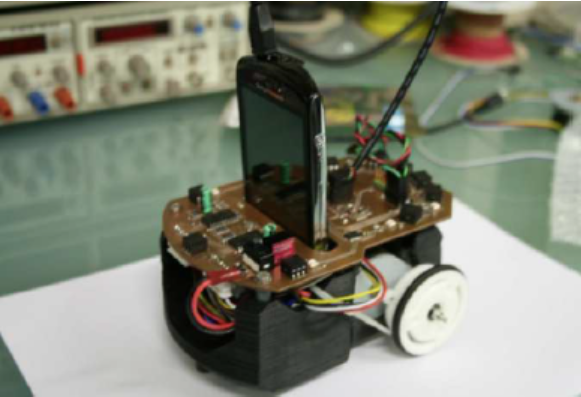
\includegraphics[width=0.8\linewidth]{imagenes/robobo1_0.PNG}
	\caption{Robobo 1.0}
	\label{fig:robobo_1_0}
\end{figure}

La primera versión de la plataforma  desarrollada por el GII fue el ROBOBO 1.0 (Figura \ref{fig:robobo_1_0}), que sirvió como versión conceptual para comprobar la viabilidad del sistema plataforma + smartphone, y presentaba las siguientes características:

\begin{itemize}

	\item 9 LEDs (diodos emisores de luz) RGB para interactuar con el usuario, que cambiaban de color con la proximidad de objetos.
	\item 9 sensores IR de proximidad para proporcionar capacidad de movimiento autónomo: 2 en la parte frontal, 4 en los laterales y los últimos tres en la parte trasera; de manera que proporcionaba una visión general del entorno.
	\item 2 motores paso a paso (convierten impulsos eléctricos en desplazamientos angulares discretos, es decir, pueden avanzar un ángulo concreto en función de la señal recibida) que aplicaban movimiento a las ruedas, con un paso de 1/8, con gran precisión de giro.
	\item Compatibilidad con dispositivos Android.
	\item Capacidad de interacción con otros dispositivos ROS.
	\item Conexión USB para la comunicación con el teléfono inteligente.

\end{itemize}

\subsection{Robobo 2.0}
\begin{figure}
	\centering
	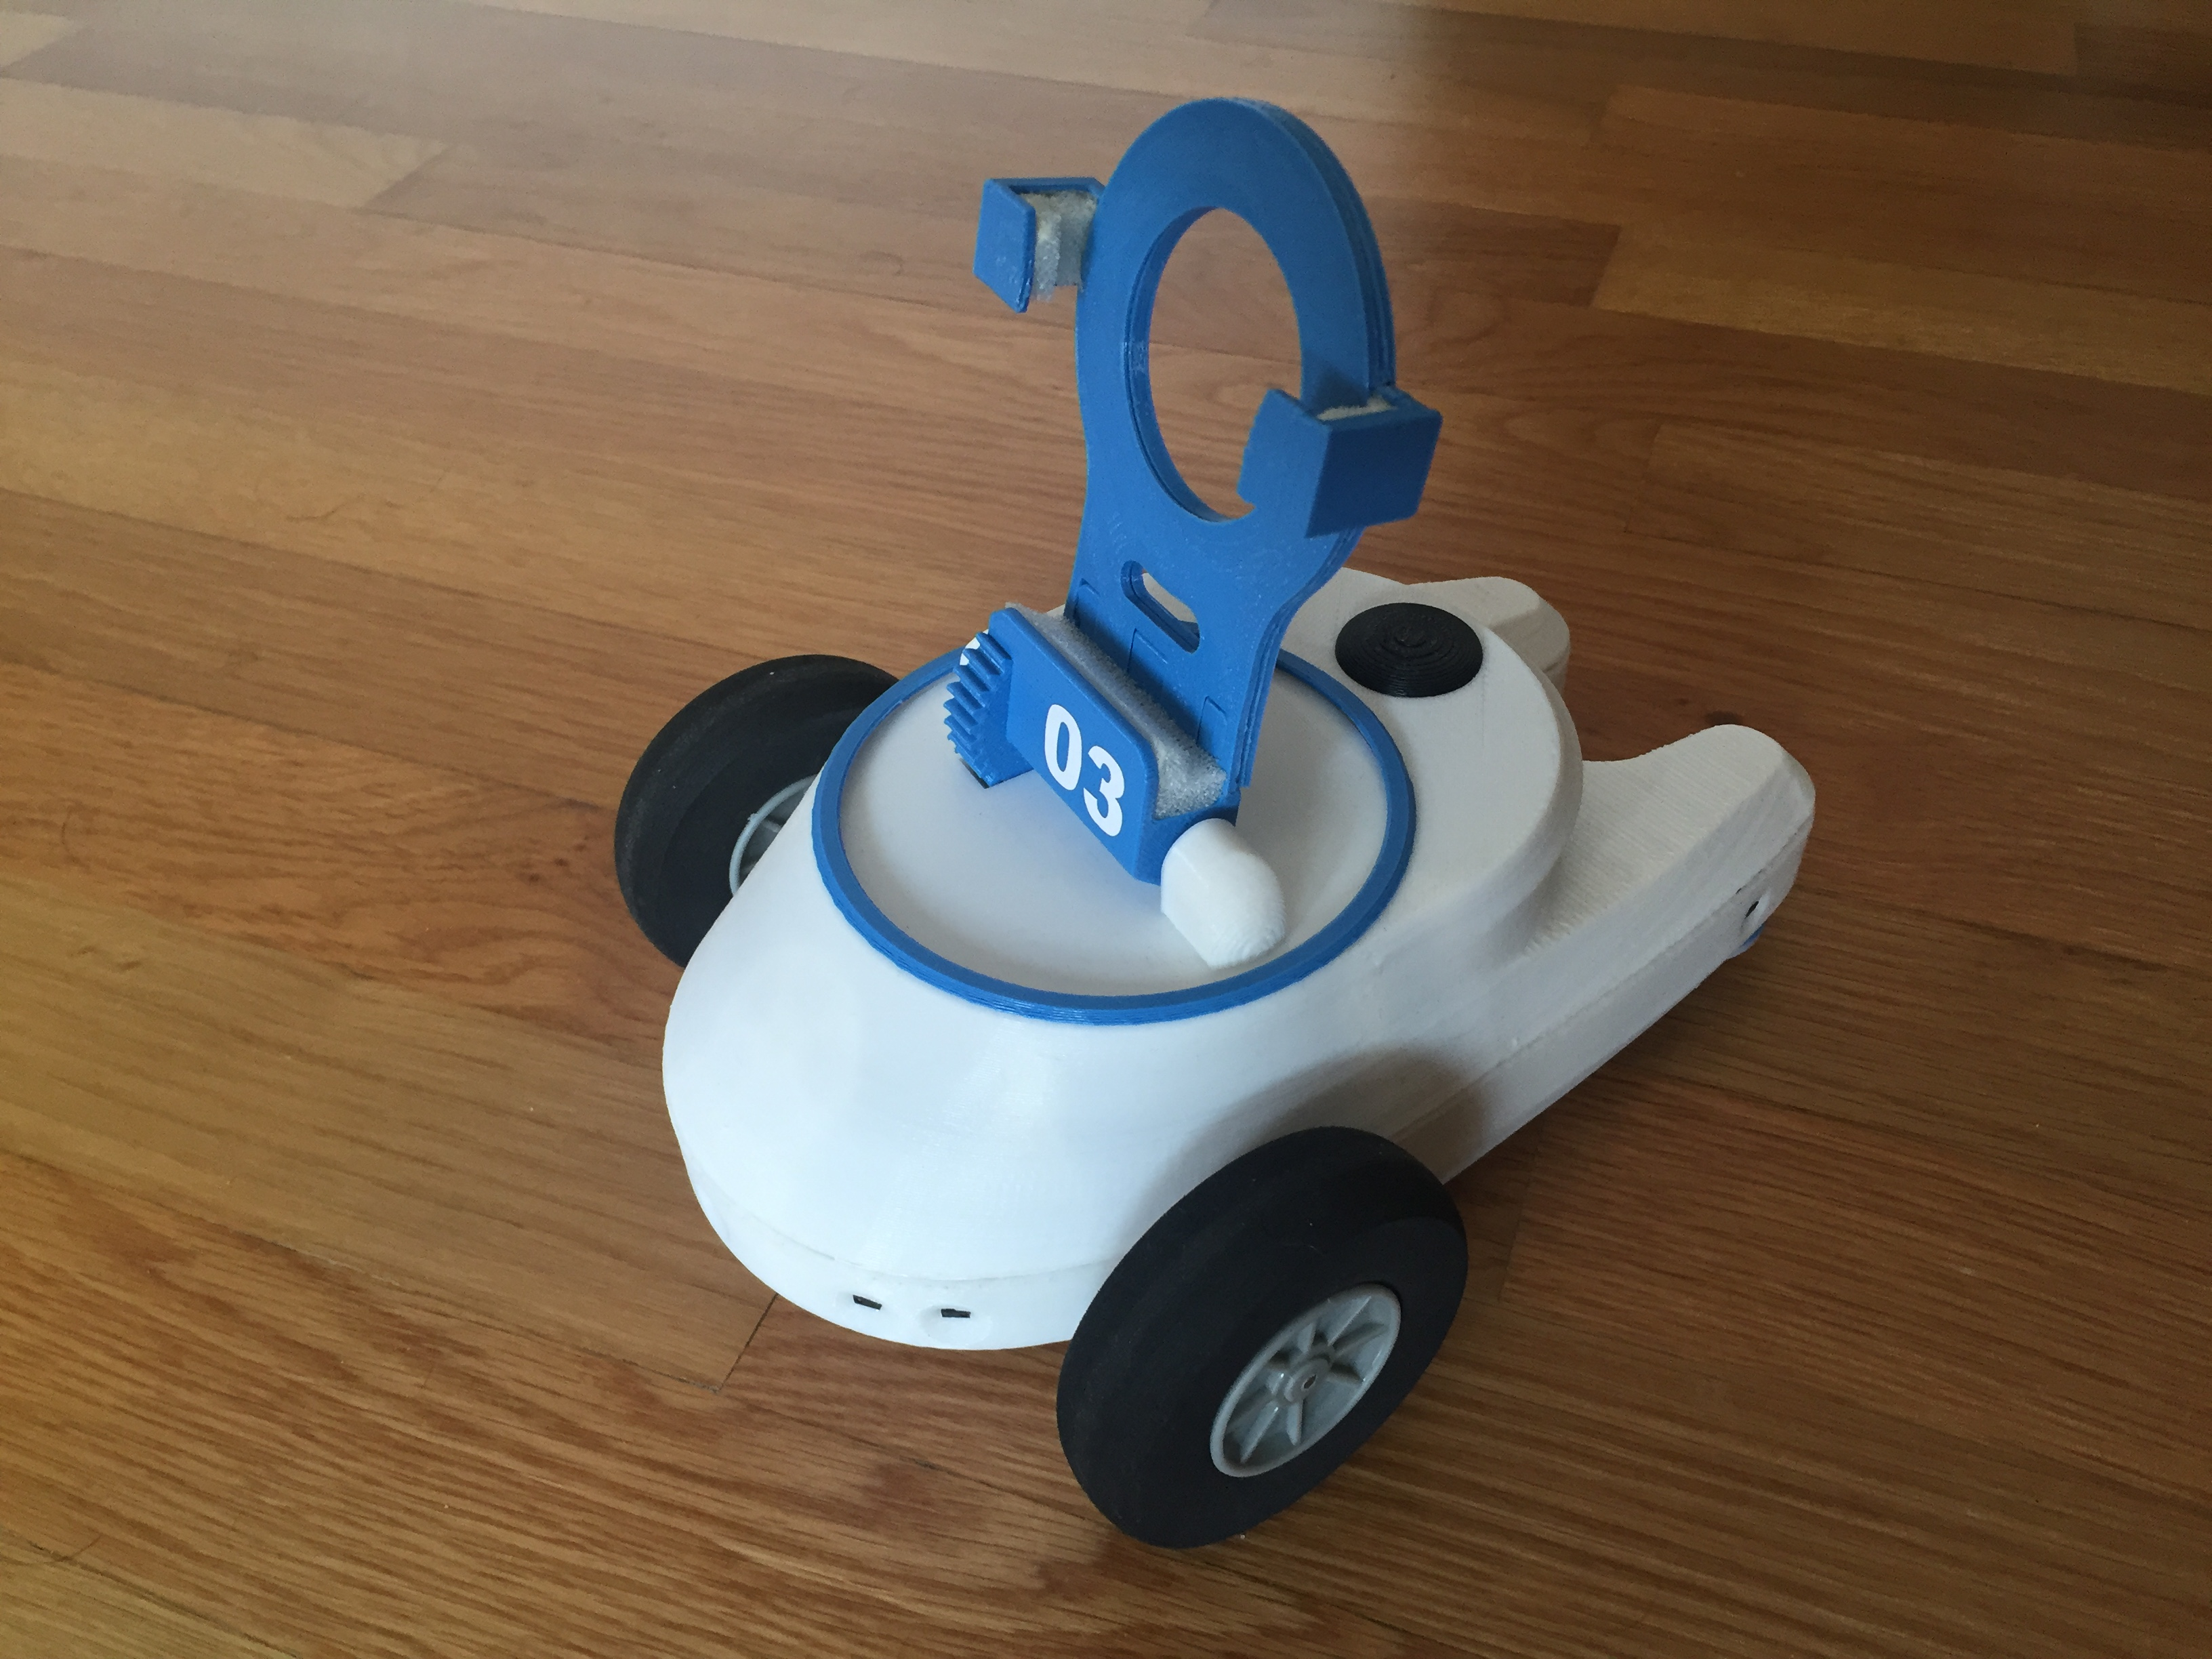
\includegraphics[width=0.8\linewidth]{imagenes/robobo_rob.JPG}
	\caption{Robobo 2.0}
	\label{fig:robobo_2_0}
\end{figure} 

La segunda versión, el ROBOBO 2.0 (figura \ref{fig:robobo_2_0}), trata de solventar las carencias de la primera versión y añadir ciertas mejoras. Tras este rediseño, las características del robot pasaron a ser:

\begin{itemize}	
%todo los leds son 9?

	\item LEDs: pasan a ser 21, 9 de ellos formando una matriz de comunicación para dar una información avanzada mediante colores y formas.
	\item Motores de las ruedas: Pasan a ser motores de corriente continua, menos voluminosos y más eficientes energéticamente. Cada motor cuenta con un encoder magnético, que transforma el movimiento del motor en pulsos eléctricos, que pueden ser interpretados por la parte software del robot.
	\item Comunicación: Se elimina la comunicación USB a favor de una conexión Bluetooth, lo cual permite utilizar diferentes smartphones con distintas posiciones de los puertos.
	\item Plataforma universal para smartphones: Se incluye un adaptador universal para teléfonos móviles, montado sobre una plataforma motorizada que permite el movimiento del smartphone sobre el chasis del robot. Esta plataforma tiene dos grados de libertad, rotación e inclinación.
	\item Sensores: Modificadas tanto el tipo, la cantidad y la posición. Se colocaron en la siguiente disposición (figura \ref{fig:robobo_2_0_sensors}):
	\begin{figure}
	\centering
	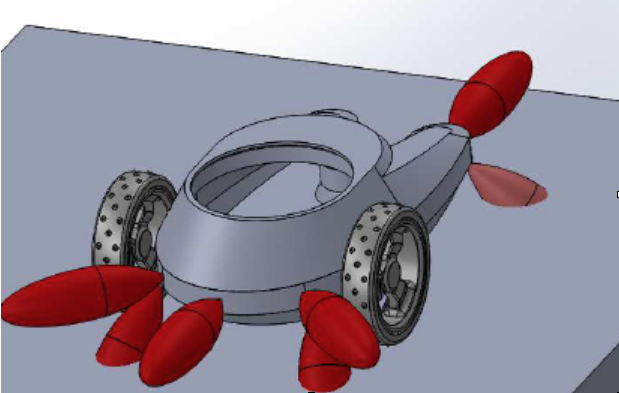
\includegraphics[width=0.8\linewidth]{imagenes/robobo_2_sensors.png}
	\caption{Disposición de los sensores en el ROBOBO 2.0}
	\label{fig:robobo_2_0_sensors}
\end{figure} 
	\begin{itemize}
	\item 3 sensores para la detección de colisiones en la parte delantera; uno frontal y los otros dos cercanos a las ruedas, de tal forma que el ROBOBO no pudiera chocar, frontalmente con ninguna superficie.
	\item 2 sensores inclinados hacia abajo para la detección de caídas, en la parte delantera, colocados cerca de las ruedas, es decir, la zona con mayor peligro de caídas.
	\item 2 sensores de caídas y 2 de colisiones, de forma similar a los anteriores, en la zona anterior del robot. 
	
	\end{itemize}
	\item Unión sensores-microcontrolador: se han cambiado las resistencias pull-up anteriores por un multiplexor. Se consigue, así, un único elemento de muchas entradas y una única salida capaz de permitir la transmisión de una, y solo una, de las entradas hacia la salida.

	\item Microcontrolador: PIC32MX534F064H, de la familia de microcontroladores de 32 bits, económico, con alta capacidad de procesamiento, diversidad de interfaces de comunicación y multitud de puertos de entrada y salida; además de que su entorno de desarrollo y su compilador son gratuitos. Este microcontrolador se programa mediante el protocolo de comunicación I2C y logra el contacto entre sensores y microcontrolador mediante buses línea de reloj “SCL” y buses línea de datos “SDA”.




\end{itemize}

Esta versión del ROBOBO, aún en pleno desarrollo, es la que se utilizará en este trabajo de final de grado que se centrará en el desarrollo de  librerías de interacción básica entre el robot y humanos, enfocándose específicamente en interacción por voz, táctil, sonido e imagen, dando lugar a módulos simples que más tarde podrán se combinados en comportamientos interactivos más complejos. El desarrollo fundamental de este trabajo se realizará en Android, ya que inicialmente el ROBOBO solo soportará teléfonos con este sistema operativo. 

%Para terminar este punto 1.1 de Motivación, deberías comentar que la versión 2.0 está en pleno desarrollo y poner algo parecido a lo que pusimos en el anteproyecto:
%En este trabajo Fin de Grado se deberán implementar diversas librerías de interacción básica del robot con humanos, centradas fundamentalmente en interacción por voz, imagen y gestos con el smartphone. El desarrollo fundamental de este trabajo se realizará en Android, ya que inicialmente el ROBOBO solo soportará teléfonos con este sistema operativo. Se comenzará por desarrollar módulos de interacción simples que más tarde serán combinados para dar lugar a comportamientos interactivos más complejos.
%Durante el desarrollo de estas librerías podrá ser necesaria la interacción con el software de control de bajo nivel de la plataforma, de modo que se ajuste este a los requerimientos de los comportamientos más complejos.

 \section{Objetivos}
 \label{sec:intro-objetives}
 El objetivo de este proyecto, como se comentó en la sección anterior, es el desarrollo de librerías que permitan una interacción básica entre el ROBOBO y humanos. Estas librerías serán desarrolladas en Android, sistema operativo que soporta el ROBOBO a día de hoy. Se desarrollarán 5 librerías Android, cada una enfocada a un tipo de interacción diferente con el robot:
 \begin{itemize}
 	\item Librería de interacción por voz
 	\item Librería de interacción por sonido
 	\item Librería de interacción táctil
 	\item Librería de interacción por imagen
 	\item Librería de interacción mediante mensajes
 \end{itemize} 
 Finalmente se implementarán una serie de ejemplos para demostrar el funcionamiento de las diferentes librerías de forma conjunta.
  %A continuación vendría el apartado 1.2 donde pones el objetivo global y los sub-objetivos en que se divide
 \section{Estructura de la memoria}
 \label{sec:intro-memory-structure}
 La memoria del trabajo está estructurada en 6 capítulos, siendo el primero de ellos esta introducción.
 \begin{itemize}
 	\item Segundo capítulo: \textbf{\textit{Fundamentos teóricos}}, se habla sobre el ROBOBO! Framework, marco de desarrollo empleado para el desarrollo de los módulos que componen este trabajo, cómo interactúa con las diferentes partes del sistema ROBOBO y las tecnologías en las que se basa.
 	
 	\item Tercer capítulo: \textbf{\textit{Antecedentes}}, se hablará sobre el campo de la interacción humano robot y se expondrán ejemplos de los diferentes modos de interacción que surgen en los diferentes campos de la robótica. 
 	\item Cuarto capítulo: \textbf{\textit{Fundamentos Tecnológicos}} se dará un repaso a las diferentes tecnologías empleadas a la hora del desarrollo de los módulos de interacción.
 	
 	\item Quinto capítulo: \textbf{\textit{Desarrollo}}, se elabora el desarrollo técnico del trabajo, el modelo conceptual, la arquitectura escogida, la metodología seguida y los detalles de implementación. 
 	
 	\item Sexto capítulo: \textbf{\textit{Resultados y pruebas}}, se comentan los resultados del desarrollo y se exponen las aplicaciones de ejemplo desarrolladas utilizando los módulos de interacción. También se exponen los problemas conocidos aún sin solución.
 
 	\item Séptimo capítulo: \textbf{\textit{Conclusiones}}, en este último capítulo se comenta el resultado general del trabajo así como el trabajo futuro a desarrollar.


 \end{itemize}
 
 \section{Herramientas utilizadas}
  \label{sec:intro-tools}
 Para el desarrollo de las librerías y aplicaciones Android que conforman el presente trabajo, se ha empleado el entorno de desarrollo \textbf{Android Studio}, basado en el IntelliJ IDEA de Jetbrains. Actualmente Android Studio es el entorno de desarrollo oficial para Android.
 
 Para la creación de los diagramas se ha empleado el software \textbf{StarUML}.
 
 Para la redacción de la memoria se ha empleado el software \textbf{Texpad}.
 
 
 
  
 
 
 % Finalmente deberías hacer un apartado 1.3 donde comentas la estructura de la memoria, sobre todo del apartado de desarrollo y pruebas



 \chapter{Contextualización}
\label{chap:contextualizacion}
\vspace{0.5cm}

%%%%%%%%%%%%%%%%%%%%%%%%%%%%%%%%%%%%%%%%%%%%%%%%%%%%%%%%%%%%%%%%%%%%%%%%%%%%%%%%
% Objetivo: Contar cómo estaba la situación antes de empezar,                  %
%           t0do lo que se hizo para familiarizarse con las tecnologías,       %
%           casarlas, etc.                                                     %
%%%%%%%%%%%%%%%%%%%%%%%%%%%%%%%%%%%%%%%%%%%%%%%%%%%%%%%%%%%%%%%%%%%%%%%%%%%%%%%%

\lettrine{E}{n} este capitulo se introducen los conceptos necesarios para la contextualización del trabajo. Se hablará sobre el proyecto D.R.E.A.M.\cite{dream_project} en el que se enmarca el proyecto ROBOBO, y sobre el trabajo previo en el robot.


\section{Proyecto D.R.E.A.M.}
\label{sec:dreamproyect}
%todo Pedir info sobre esto (Dream)
Este trabajo fin de grado se enmarca dentro del proyecto europeo de investigación DREAM (Deferred Restructuring of Experience in Autonomous Machines) que se lleva a cabo en el Grupo Integrado de Ingeniería (GII). El objetivo global de dicho proyecto consiste en el desarrollo de una arquitectura cognitiva que permita a los dispositivos robóticos realizar tareas de aprendizaje y optimización de sus comportamientos. En particular, estas tareas se realizarán tanto durante el período de actividad como durante el período de inactividad de los robots (aprendizaje en fase de sueño) en analogía al funcionamiento del cerebro en lo seres humanos durante los períodos de sueño.

\section{Plataforma ROBOBO 2.0}
\label{sec:roboboplatform}

\begin{figure}
	\centering
	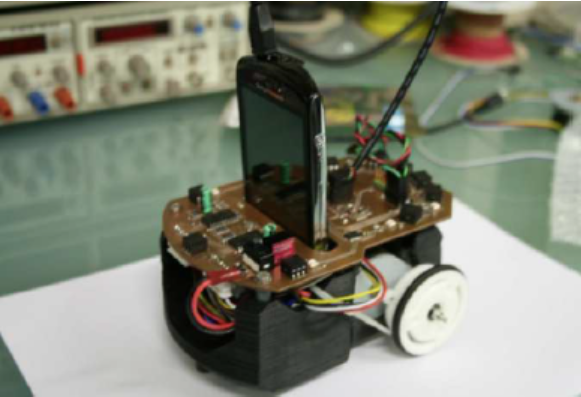
\includegraphics[width=0.8\linewidth]{imagenes/robobo1_0.PNG}
	\caption{Robobo 1.0}
	\label{fig:robobo_1_0}
\end{figure}

La primera versión de la plataforma fue desarrollada por el Grupo Integrado de Ingeniería de la UDC, el ROBOBO 1.0 (Figura \ref{fig:robobo_1_0}) , sirvió como versión conceptual para comprobar la factibilidad del sistema plataforma + smartphone, y presentaba las siguientes características:

\begin{itemize}

	\item 9 LEDs (diodos emisores de luz) RGB para interactuar con el usuario, que cambiaban de color con la proximidad de objetos.
	\item 9 sensores IR de proximidad para proporcionar capacidad de movimiento autónomo: 2 en la parte frontal, 4 en los laterales y los últimos tres en la parte trasera; de manera que proporcionaba una visión general del entorno.
	\item 2 motores paso a paso (convierten impulsos eléctricos en desplazamientos angulares discretos, es decir, pueden avanzar un ángulo concreto en función de la señal recibida) que aplicaban movimiento a las ruedas, con un paso de 1/8, con gran precisión de giro.
	\item Compatibilidad con dispositivos Android.
	\item Capacidad de interacción con otros dispositivos ROS.
	\item Conexión USB para la comunicación con el teléfono inteligente.

\end{itemize}


\begin{figure}
	\centering
	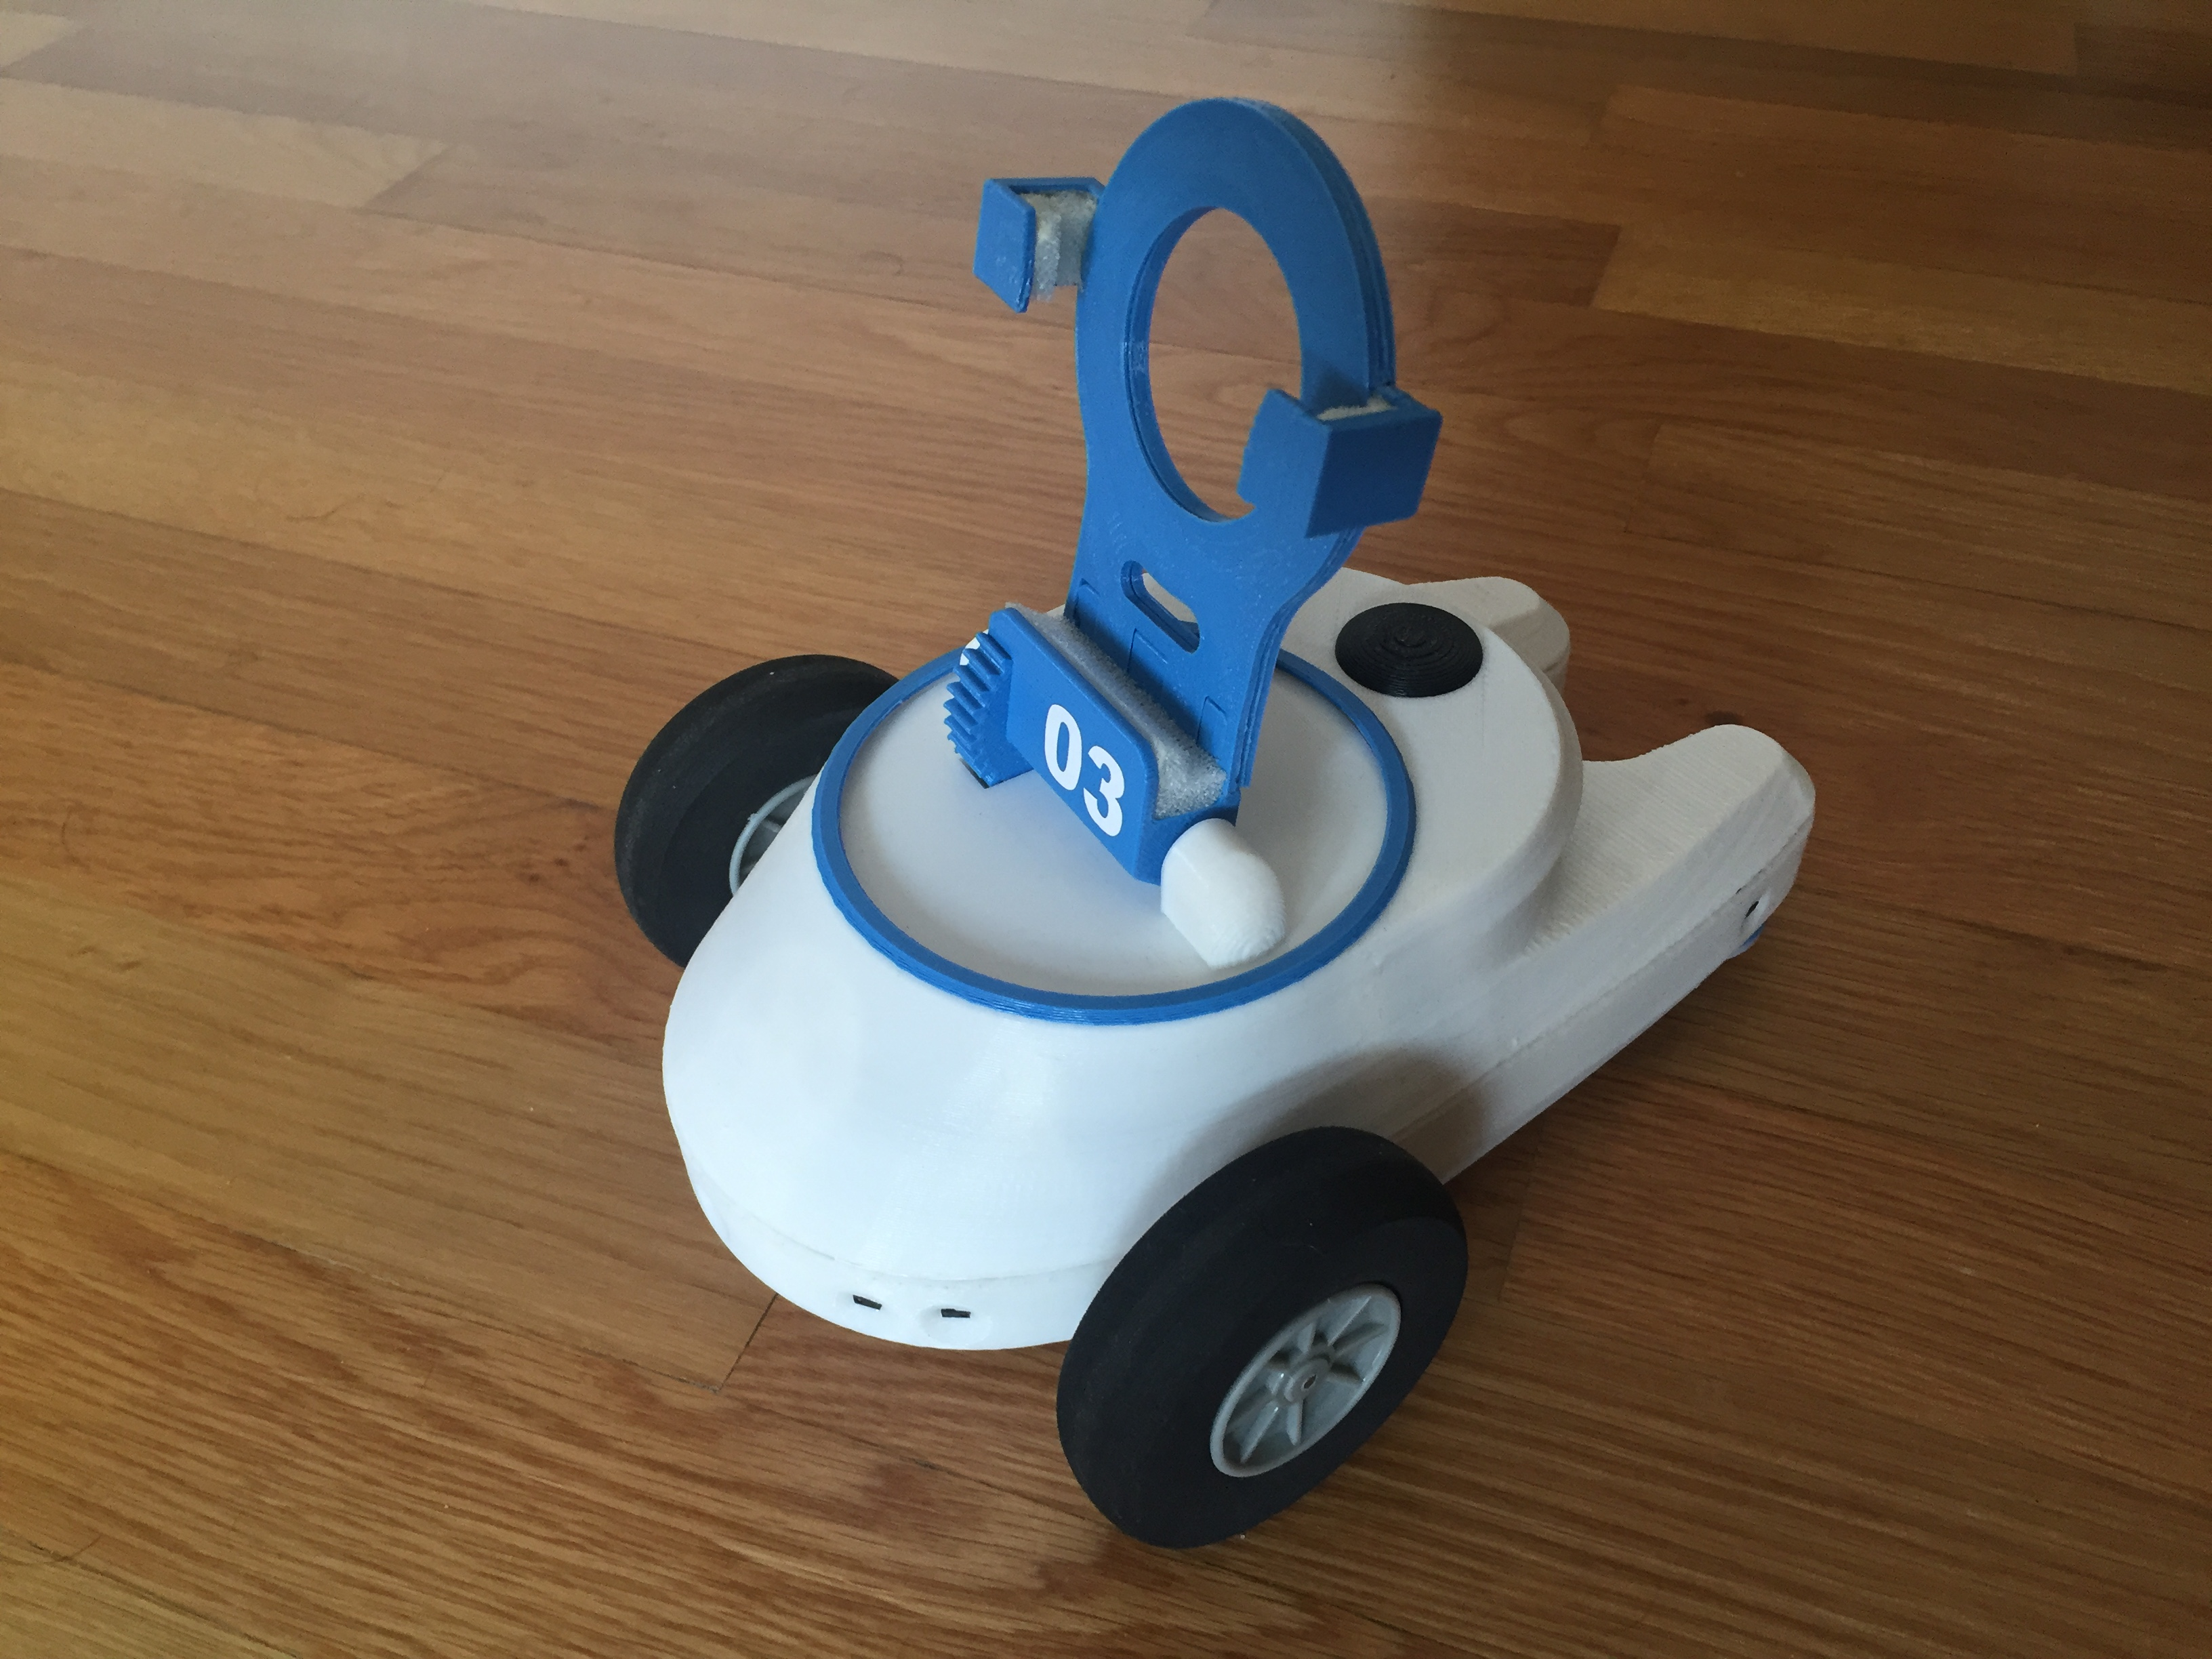
\includegraphics[width=0.8\linewidth]{imagenes/robobo_rob.JPG}
	\caption{Robobo 2.0}
	\label{fig:robobo_2_0}
\end{figure} 

La segunda versión, el ROBOBO 2.0 (figura \ref{fig:robobo_2_0}) , fue desarrollada para solventar las carencias de la primera versión y añadir ciertas mejoras. Tras este rediseño, las características del robot pasaron a ser:

\begin{itemize}
	\item LEDs: pasan a ser 21, 9 de ellos formando una matriz de comunicación para dar una información avanzada mediante colores y formas.
	\item Motores de las ruedas: Pasan a ser motores de corriente continua, menos voluminosos y más eficientes energéticamente. Cada motor cuenta con un encoder magnético, que transforma el movimiento del motor en pulsos eléctricos, que pueden ser interpretados por la parte software del robot.
	\item Comunicación: Se elimina la comunicación USB a favor de una conexión Bluetooth, lo cual permite utilizar diferentes smartphones con distintas posiciones de los puertos.
	\item Plataforma universal para smartphones: Se incluye un adaptador universal para teléfonos moviles, montado sobre una plataforma motorizada que permite el movimiento del snartphone sobre el chasis del robot. Esta plataforma tiene dos grados de libertad, rotación e inclinación.
	\item Sensores: Modificadas tanto el tipo, la cantidad y la posición. Se colocarón en la siguiente disposición (figura \ref{fig:robobo_2_0_sensors}):
	\item \begin{figure}
	\centering
	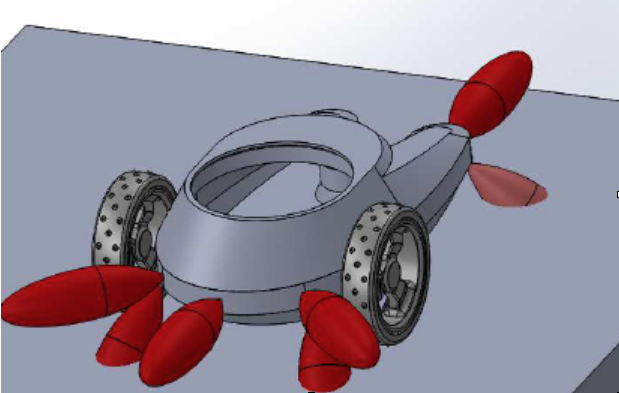
\includegraphics[width=0.8\linewidth]{imagenes/robobo_2_sensors.png}
	\caption{Disposición de los sensores en el ROBOBO 2.0}
	\label{fig:robobo_2_0_sensors}
\end{figure} 
	\begin{itemize}
	\item 3 sensores para la detección de colisiones en la parte delantera; uno frontal y los otros dos cercanos a las ruedas, de tal forma que el ROBOBO no pudiera chocar, frontalmente con ninguna superficie.
	\item 2 sensores inclinados hacia abajo para la detección de caídas, en la parte delantera, colocados cerca de las ruedas, es decir, la zona con mayor peligro de caídas.
	\item 2 sensores de caídas y 2 de colisiones, de forma similar a los anteriores, en la zona anterior del robot. 
	
	\end{itemize}
	\item Unión sensores-microcontrolador: se han cambiado las resistencias pull-up anteriores por un multiplexor. Se consigue, así, un único elemento de muchas entradas y una única salida capaz de permitir la transmisión de una, y solo una, de las entradas hacia la salida.

	\item Microcontrolador: PIC32MX534F064H, de la familia de microcontroladores de 32 bits, económico, con alta capacidad de procesamiento, diversidad de interfaces de comunicación y multitud de puertos de entrada y salida; además de que su entorno de desarrollo y su compilador son gratuitos. Este microcontrolador se programa mediante el protocolo de comunicación I2C y logra el contacto entre sensores y microcontrolador mediante buses línea de reloj “SCL” y buses línea de datos “SDA”.




\end{itemize}




\subsection{ROBOBO! Framework}

\begin{figure}
	\centering
	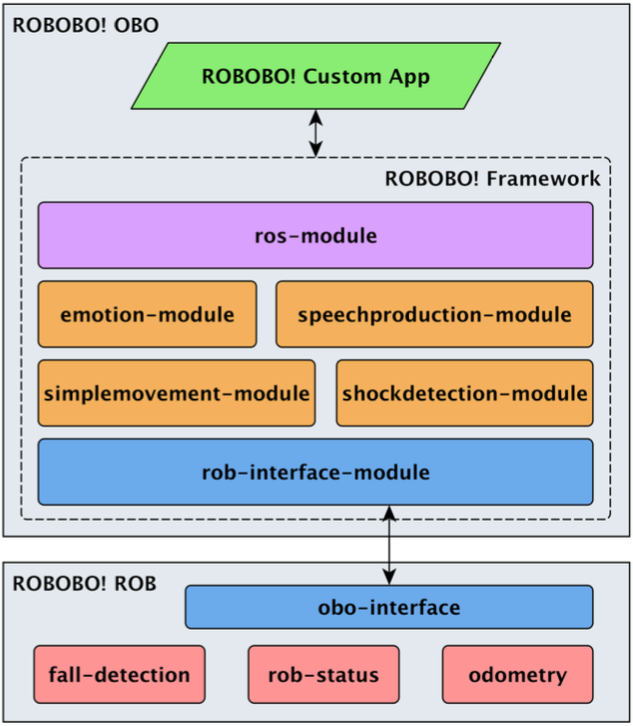
\includegraphics[width=0.6\linewidth]{imagenes/robobo_framework.png}
	\caption{Estructura de ROBOBO! framework dentro del entorno ROBOBO}
	\label{fig:robobo_framework_estructure}
\end{figure}

El ROBOBO! Framework\cite{RoboboFramework} es el framework de desarrollo usado para desarrollas aplicaciones para el ROBOBO. Está diseñado de manera modular, de forma que facilita la extensión del mismo con nuevos módulos. Está publicado con una licencia libre LGPL v3.
Ofrece el módulo \textit{rob-interface-module}, que permite la comunicación entre la plataforma robotizada (denominada ROB, figura \ref{fig:robobo_2_0}) y el smartphone (denominado OBO en el sistema). También proporciona el módulo \textit{ros-module} que sirve de interfaz entre el robot y ROS \cite{Ros}










 
 \chapter{Interacción Humano Robot}
\label{chap:interaccion-humano-robot}

%%%%%%%%%%%%%%%%%%%%%%%%%%%%%%%%%%%%%%%%%%%%%%%%%%%%%%%%%%%%%%%%%%%%%%%%%%%%%%%%
% Objetivo: Exponer de qué va este proyecto, sus líneas maestras, objetivos,   %
%           etc.                                                               %
%%%%%%%%%%%%%%%%%%%%%%%%%%%%%%%%%%%%%%%%%%%%%%%%%%%%%%%%%%%%%%%%%%%%%%%%%%%%%%%%

%todo http://humanrobotinteraction.org/human-robot-interaction-a-historical-perspective-and-current-research-trends/


%Objetivos de interacción del proyecto, modelo conceptual del mismo.

\lettrine{E}{n} este capítulo se introduce el tema de la Interacción humano robot, 	y el diseño conceptual del sistema de interacción desarrollado para la plataforma ROBOBO.

\section{Introducción}
 \label{sec:hri-intro}
 
 %todo meter lo de las conferencias
 Desde finales de la década de los 90, la interacción entre humanos y robots ha cobrado importancia, creando un nuevo campo de investigación en la ciencia\cite{goodrich2007human}, la interacción humano-robot (HRI por sus siglas en inglés). El campo de la HRI busca entender, modelar y evaluar las diferentes modalidades de interacción entre las personas y los robots. La comunicación entre humanos y robots puede dividirse  en dos categorías generales:
 \begin{itemize}
 	\item Interacción remota
 	\item Interacción próxima
 \end{itemize}
 
 La interacción remota suele ser referida como control supervisado o teleoperación, dependiendo de si el robot es autónomo con supervisión de un humano, que interviene en caso de necesidad, o si el robot es controlado por el humano directamente. Este tipo de interacción puede verse en robots de tipo industrial o en vehículos autónomos, cómo los llamados Drones del ejercito.
 
 La interacción próxima es aquella en la que el robot interactúa directamente con el humano, llegando incluso a haber interacción física. Este tipo de interacción incluye elementos emotivos y sociales, y se puede encontrar en, por ejemplo, los robots asistenciales o educativos. Este tipo de interacción es la que se tratará en este trabajo, en el cual se diseñarán diferentes sistemas de interacción para la plataforma ROBOBO.
 
 \subsection{HRI en la industria}
 
 Generalmente, en los procesos industriales, la interacción entre los robots y los operadores suele ser remota, los sistemas se programan para realizar una tarea y el humano solamente interviene en caso de necesidad, sin embargo pueden darse casos de interacción próxima con los robots. Uno de estos casos podría ser el aprendizaje de tareas mediante demostración, proceso mediante el cual, un operador humano realiza una tarea, por ejemplo moviendo manualmente el brazo de un robot, para que el controlador aprenda a realizar esa tarea. Este tipo de interacción permite que los robots aprendan comportamientos de alto nivel difícilmente programables.\\
 Sin embargo a la hora de realizar tareas de forma cooperativa entre robots y humanos, la interacción cercana con robots industriales conlleva riesgos importantes, como pudo verse en el accidente del 2015\cite{vwaccident2015} en la planta de Volkswagen cerca de Kassel, Alemania, en el que un operario fué golpeado por un brazo industrial  durante su instalación, resultando en la muerte del técnico.
  \begin{figure}
	\centering
	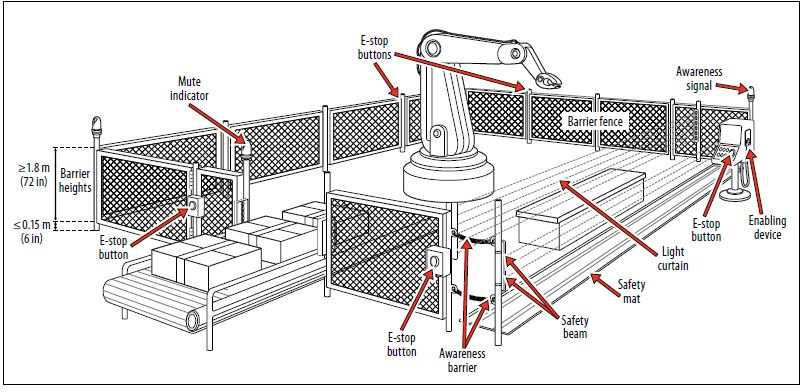
\includegraphics[width=1\linewidth]{imagenes/robotcell.jpeg}
	\caption{Esquema de una jaula de seguridad para un robot industrial}
	\label{fig:robot-cell}
\end{figure} 
 Para evitar esta clase de accidentes, se está buscando la consciencia del entorno en los manipuladores robóticos, para poder adaptar sus reacciones al contexto actual. Este tipo de consciencia no solo disminuye los riesgos de operación, sino que también disminuye espaciales, ya que los robots no requerirían de jaulas de seguridad (figura \ref{fig:robot-cell}) , también la productividad se vería afectada positivamente, ya que tareas imposibles de realizar para un robot y para un humano individualmente, pueden llevarse a cabo mediante la llamada robótica cooperativa.
 En \textit{Cooperative Tasks between Humans and Robots in Industrial Environments}\cite{corrales2012cooperative} presentan un sistema de robótica cooperativa en el que un operador y un robot colaboran de manera cercana para llevar a cabo diferentes tareas, de manera que el robot realiza las tareas repetitivas y peligrosas, mientras que el humano lleva a cabo las tareas que requieren de cierta precisión o inteligencia con la que no cuenta el robot. En este sistema el operador lleva un traje de posicionamiento, que permite al robot conocer su posición, pudiendo así adaptar sus movimientos de manera que el humano no corra riesgos.
 
 
 
 \subsection{HRI en robots asistenciales}
 Uno de los campos en los que la interacción entre humanos y robots cobra mucha importancia es en el nicho de los robots asistenciales. Los robots asistenciales, también llamados de servicio, son definidos por la federación internacional de robótica cómo \textit{Robots que operan de forma total o semiautónoma para realizar servicios útiles para el bienestar de humanos y equipamiento, excluyendo las operaciones de manufactura}\cite{ifr-service-robots}. En esta definición se diferencia entre dos tipos de robots asistenciales:
 \begin{itemize}
 	\item Robots personales
 	\item Robots profesionales
 \end{itemize}
 
 Los robots personales son aquellos que se utilizan para labores no comerciales, generalmente por personas sin perfil técnico. Por ejemplo, sillas de ruedas eléctricas, robots de asistencia de movilidad, o aspiradoras automáticas.
 
 Los robots profesionales son aquellos utilizados para realizar tareas de asistencia en un entorno comercial, generalmente manejados y supervisados por un personal especializado. Por ejemplo robots de limpieza automatizados para zonas públicas, robots de mensajería en oficinas u hospitales, robots anti-incendios,robots quirúrgicos y de rehabilitación en hospitales o los robots terapéuticos.
 \begin{figure}
	\centering
	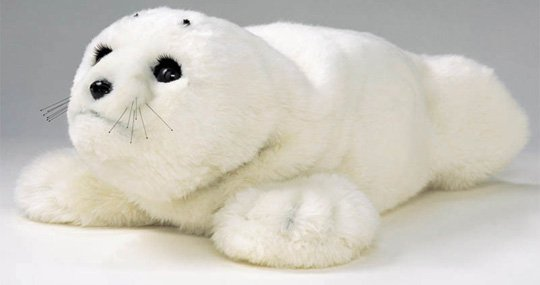
\includegraphics[width=0.8\linewidth]{imagenes/parorobot.JPG}
	\caption{Robot terapeutico Paro}
	\label{fig:parorobot}
\end{figure} 

 En los robots terapéuticos se pueden encontrar múltiples formas de interacción, por ejemplo, el robot Paro\cite{parorobots} (figura \ref{fig:parorobot}) es un robot terapéutico con forma de bebé foca, utilizado con éxito en terapias contra la Demencia, que busca una interacción emocional con el paciente, para ello cuenta con cinco tipos de sensores diferentes, táctiles, auditivos, de temperatura, de luz y posturales. Los pacientes realizan una interacción con el robot cómo la que tendrían con un animal, y el robot responde acorde a los estímulos que recibe. Esto, en conjunto con la forma física del robot, más semejante a un animal de peluche que a una máquina, permite al paciente desarrollar emociones.
   \begin{figure}
	\centering
	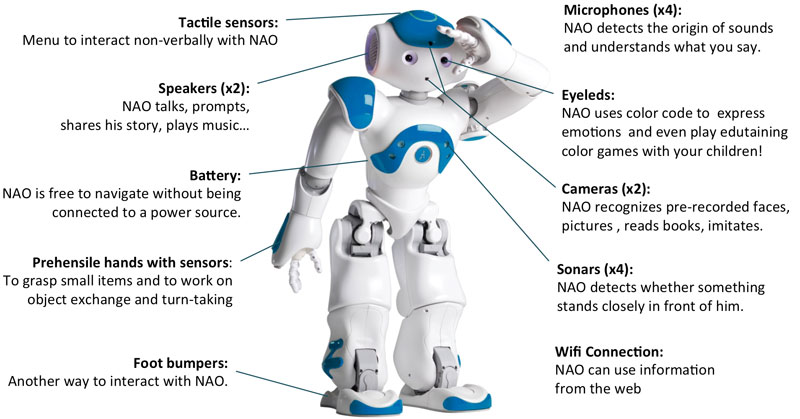
\includegraphics[width=1\linewidth]{imagenes/naorobot.jpg}
	\caption{Esquema de características del robot NAO}
	\label{fig:naorobot}
\end{figure} 
 El robot NAO\cite{naorobots}(figura \ref{fig:naorobot}) es otro de los robots que se están empleando con éxito en tareas asistenciales, tanto de manera terapéutica, como robot de relaciones publicas o para tareas de educación. El robot cuenta con una amplia variedad de sensores y actuadores que le permiten interactuar de diversas formas con el usuario:
 \begin{itemize}
 	\item Cámaras: Permiten reconocimiento de caras y procesado de imagen.
 	\item Sensores táctiles y de presión: Permiten una interacción física con el robot.
 	\item Altavoces: Permiten al robot producir diversos sonidos y hablar.
 	\item Micrófonos: Permiten reconocer habla y ubicar el origen de los sonidos espacialmente.
 	\item Sensores de distancia: Permiten detectar la distancia a los objetos.
 	\item 25 Grados de libertad: Permiten al robot interactuar fisicamente con su entorno y realizar comunicación no verbal.
 	\item Unidad de medición inercial: Permite detectar aceleraciones y giros.
 \end{itemize}
\begin{figure}
	\centering
	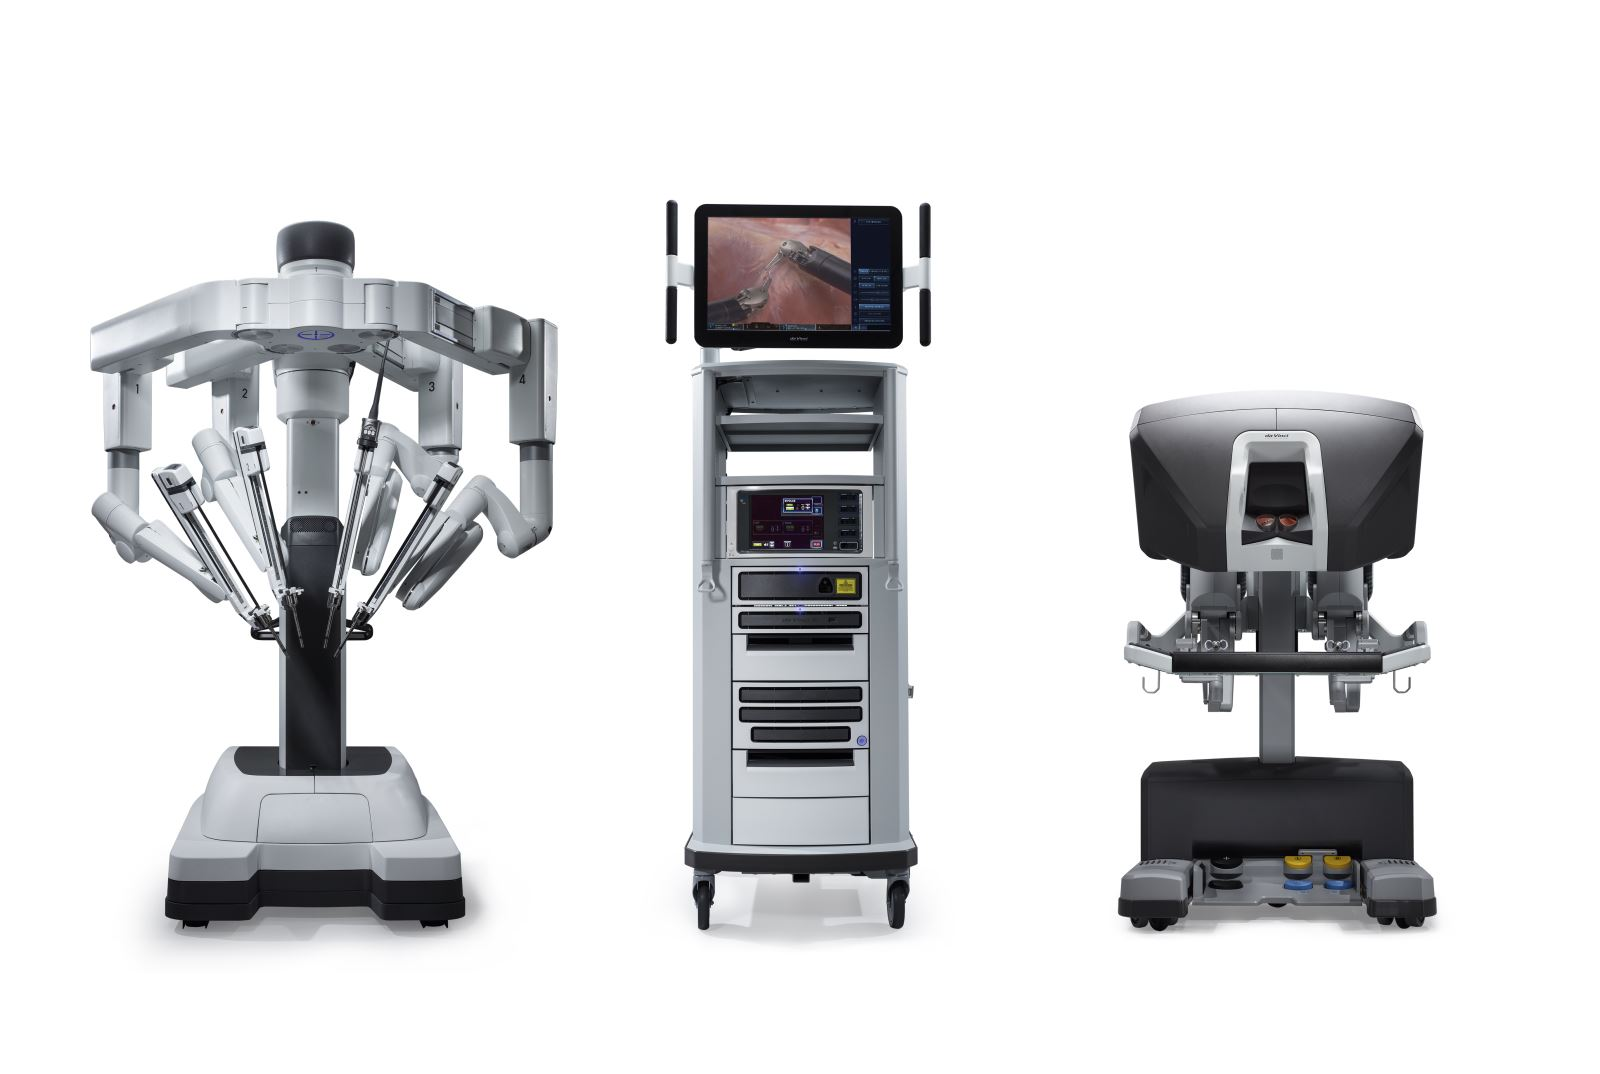
\includegraphics[width=1\linewidth]{imagenes/davincisystem.jpg}
	\caption{Sistema quirúrgico daVinci}
	\label{fig:davincisystem}
\end{figure} 
 
 En el caso de los robots médicos, los quirúrgicos especificamente, la interacción no suele pasar de la teleoperación del robot, es decir, el robot se controla como si fuera una extensión del cirujano. El robot más conocido en este campo es el sistema quirúrgico Da Vinci (figura \ref{fig:davincisystem}), utilizado en cirugía de precisión. En este robot el cirujano controla los diferentes brazos del aparato desde una consola que cuenta con controles con feedback háptico, es decir, el operador no mueve unicamente el brazo, sino que siente lo que hay al final del mismo, la presión ejercida y la resistencia al movimiento, dando al cirujano el tacto necesario para realizar las diferentes tareas que se realizan en una operación, como coser o cortar, de forma natural y con un alto grado de precisión.
 

 
 \subsection{HRI en robots de entretenimiento}
 Se entiende por robots de entretenimiento aquellos cuya finalidad no es más que divertir al usuario. Dentro de esta categoría podríamos incluir a los robots mascota, que generalmente realizan una interacción de alto nivel con el usuario.
 Por ejemplo, uno de los robots más relevantes en el ámbito de los robots mascota es el desarrollado por Sony, Aibo \cite{aibo} (figura \ref{fig:aiborobot}) , cuya finalidad era comportarse como un perro. En este robot podemos encontrar múltiples tipos de interacción, interacción física en forma de movimientos perrunos, reconocimiento facial a través de cámaras, a través de caricias utilizando los sensores táctiles, y en las últimas versiones del robot mediante una matriz de leds situada en la cara del aparato, que permite poner diferentes expresiones en función del "humor" del robot. Mediante todas estas capacidades motoras y sensoriales, se puede interactuar con una unidad Aibo de manera semejante a la que se tendría con un perro real.
 Otro ejemplo de mascota robótica es el Bandai SmartPet (figura \ref{fig:bandaismartpet}) , un robot pensado para utilizar junto un smartphone IPhone, que es colocado en la cabeza del robot y provee múltiples formas de interacción, reconocimiento de gestos mediante la cámara frontal, reconocimiento de sonido utilizando el micrófono y reconocimiento de gestos táctiles en la pantalla.
 
 \begin{figure}
	\centering
	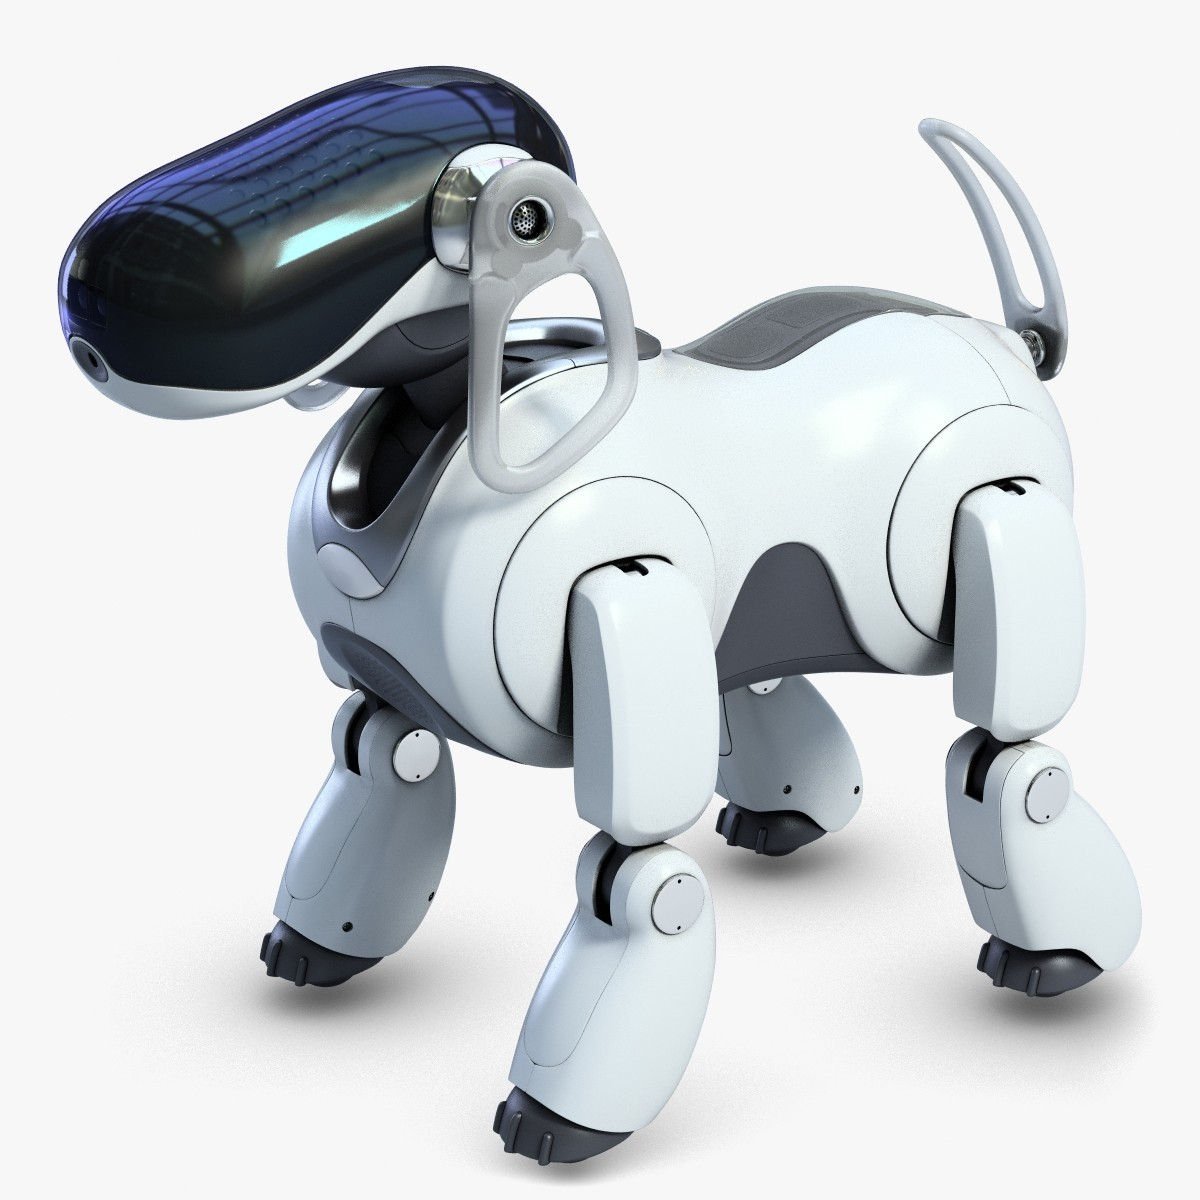
\includegraphics[width=0.5\linewidth]{imagenes/aiborobot.jpg}
	\caption{Robot mascota Aibo de Sony}
	\label{fig:aiborobot}
 \end{figure}
  \begin{figure}
	\centering
	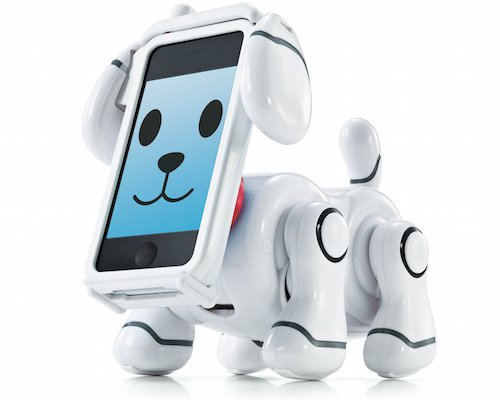
\includegraphics[width=0.5\linewidth]{imagenes/bandaismartpet.jpg}
	\caption{Robot mascota Smartpet de Bandai}
	\label{fig:bandaismartpet}
 \end{figure}

 \subsection{HRI en robots educativos}
 En  los últimos años el uso de robots con fines educativos, si bien ya eran usados de manera educativa en enseñanza superior, ha tomado impulso en la educación primaria y secundaria, apareciendo múltiples robots enfocados a este tipo de mercado. La interacción con esta clase de robots puede darse de diferentes formas según el público objetivo, dependiendo principalmente del rango de edades del mismo.

\begin{figure}
\centering
\begin{minipage}{0.45\textwidth}
\centering
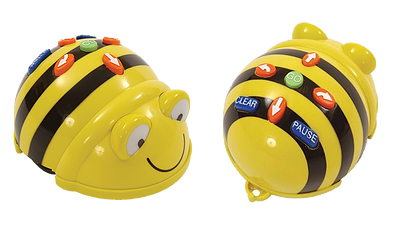
\includegraphics[width=1\linewidth]{imagenes/beebot.png}
\caption{Beebot}
\label{fig:beebot}

\end{minipage}\hfill
\begin{minipage}{0.45\textwidth}
\centering
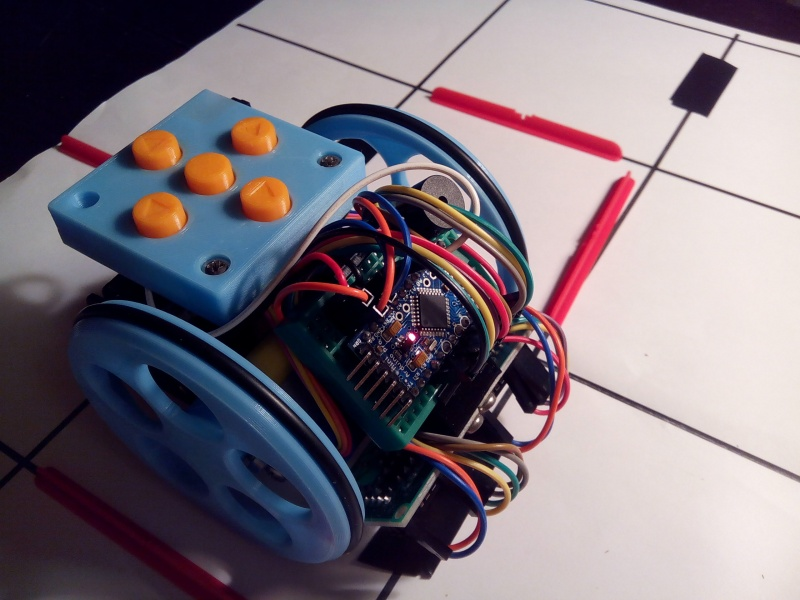
\includegraphics[width=1\linewidth]{imagenes/escornabot.jpg}

\caption{Escornabot}
\label{fig:escornabot}

\end{minipage}
\end{figure}

 Enfocados a la educación infantil nos podemos encontrar con robots cómo el BeeBot(figura \ref{fig:beebot}) o su alternativa libre, el Escornabot(figura \ref{fig:escornabot}),la finalidad de estos robots es la introducción a los niños a la programación, en forma de pensamiento secuencial, y a la resolución de problemas. En esta clase de robots la interacción está limitada a la introducción de comandos en la botonera de la parte superior del robot, que serán traducidos a movimientos del robot posteriormente.  

 En la educación primaria y secundaria los robots utilizados ya adquieren una mayor complejidad y suelen emplearse para una introducción real a la programación, generalmente utilizando lenguajes gráficos de muy alto nivel como Scratch\cite{scratch}. Uno de los robots más relevantes en este ámbito es el kit Mindstorms de Lego (figura \ref{fig:legoev3}) , que no solo permite programar el robot, sino también construirlo. El Lego Mindstorms cuenta con diferentes sensores y actuadores que ofrecen diversas maneras de interacción con el robot:
 \begin{itemize}
 	\item Motores: Permiten el movimiento del robot de manera relativamente precisa
 	\item Sensores de distancia: Permiten medir distancias y actuar en consecuencia a los datos medidos
 	\item Sensores de luz ambiente: Miden la intensidad de la luz del entorno
 	\item Sensores de color: Permiten detectar los colores básicos
 	\item Unidad inercial: Permite medir giros en el plano horizontal
 \end{itemize}
 
   \begin{figure}
	\centering
	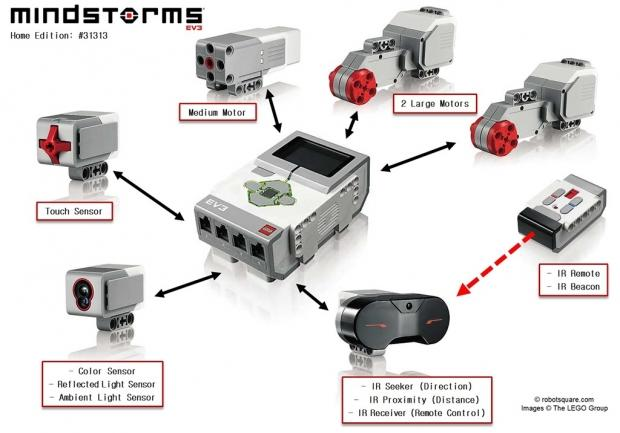
\includegraphics[width=0.8\linewidth]{imagenes/legoev3.jpg}
	\caption{Kit básico Lego Mindstorms EV3}
	\label{fig:legoev3}
\end{figure} 

En la llamada educación especial la robótica también esta siendo empleada con éxito, por ejemplo el robot NAO (figura \ref{fig:naorobot}), del que se habló en la sección anterior, se utiliza para educar a niños con trastornos de espectro autista. El éxito de este tipo de educación viene dada debido a que la interacción con el robot, al ser programada, resulta predecible para el alumno, creando un entorno estable y pautado que resulta óptimo en este tipo de trastornos. La interacción en este caso se da en forma de movimientos preprogramados y mediante los leds de los ojos del robot, que cambian de color segun las emociones que intenta expresar el robot, lo cual ayuda al alumno a ejercitar uno de las mayores dificultades dadas por el autismo, la dificultad de establecer relaciones empáticas.
 
  Ejemplos de diferentes robots y modos de interacción... Industriales, guías de museo, asistenciales, educativos
 
 \section{Interacción con robots educativos}
 \label{sec:hri-robots-educativos}
 Ejemplos específicos de robots educativos
 
 \section{Solución para el ROBOBO}
 \label{sec:hri-solucion-robobo}
 
 La plataforma ROBOBO, cuenta con características que permiten realizar diversas maneras de interacción, el hecho de estar basado en un smartphone, pone todas las capacidades del mismo a disposición a la hora de interactuar con los usuarios. Partiendo del hardware con el que se cuenta, base motorizada \textit{ROB} y smartphone \textit{OBO} , se han definido, en una analogía a los sentidos, una serie de paquetes para dotar al ROBOBO de diversas funcionalidades de interacción.
 
 El primero de estos paquetes sería el paquete de habla. Siendo el habla, probablemente, la principal forma de interacción que se da entre los humanos, parece lógico que, teniendo la capacidad de proceso de un smartphone moderno, dotar al robot ya no solo de la capacidad de producir habla, sino de entender texto hablado es un concepto interesante. Este paquete daría al robot la posibilidad de comunicación bidireccional con los humanos, además de darle al robot cierta personalidad más \enquote{orgánica} , haciéndolo más atractivo, por ejemplo, a los niños.
 
 El segundo, de forma análoga al sentido del tacto, teniendo una \enquote{piel artificial} cómo es la pantalla táctil del teléfono, dar la capacidad al robot de sentir toques y caricias parece una idea interesante a la hora de llevar una interacción cercana con el robot.
 
 El tercero, siguiendo la analogía con los sentidos, sería el sentido del oído. La capacidad de producir y reconocer sonidos abre puertas a tipos de interacción interesantes. Por ejemplo, la capacidad de reaccionar ante sonidos fuertes como palmadas o la capacidad de reconocer notas musicales podrían permitir al robot comunicarse mediante el uso de la música, y estando el ROBOBO enfocado directamente a la educación, esta clase de interacción podría emplearse para la enseñanza musical en la educación infantil y primaria.
 
 El cuarto paquete, teniendo hoy en día todos los smartphones como mínimo una cámara, busca dotar al ROBOBO de sentido de la vista. Con este sentido, el robot podría detectar la presencia de gente y a que distancia se encuentran y de esta manera adaptar su comportamiento a su entorno, por ejemplo, alejándose si nota que alguien esta muy cerca o siguiendo con la \enquote{cara} a la gente a su alrededor. La capacidad de discernir diferentes colores también es una habilidad interesante de cara a la educación de niños muy pequeños.
 
 Por último, teniendo la capacidad de conectarse a internet del smartphone, parece interesante dotar al robot de la capacidad de comunicarse a través de la red. El correo electrónico es un sistema de comunicación muy extendido y casi obligatorio hoy en día, así que, dada la extensión del sistema, y la cantidad de usuarios con los que cuenta, parece la opción correcta para este tipo de comunicación.
 
 %%todo Partir desde la plataforma, desarrollar los diferentes métodos de interacción en función de las capacidades. En función del hardware.
  

 \chapter{Fundamentos tecnológicos}
\label{chap:fundamentos-tecnologicos}

\lettrine{A}  la hora de desarrollar los módulos de  interacción, para cubrir las limitaciones de la API de Android que aun siendo extensa no proporciona funcionalidades para todo, se han empleado una serie de librerías adicionales. 

En este capítulo se explicarán brevemente estas librerías y su rol dentro del subsistema de interacción desarrollado en este trabajo.
 \section{Sphinx}
 \label{subsec:sphinx}

 
 CMU Sphinx\cite{cmusphinx} es una serie de sistemas de reconocimiento de voz desarrollados en la Universidad de Carnegie Mellon.
 En este trabajo se emplea una versión ligera de Sphinx adaptada a dispositivos móviles, Pocket Sphinx, con el modelo acústico y el diccionario para el idioma inglés.
 
 La capacidad de reconocer voz sin la necesidad de una conexión a internet constante favoreció a esta librería frente a otras, como podría ser el sistema de reconocimiento vocal de Google.
 
 Esta librería se ha usado para implementar el módulo de detección de habla, que se explica con detenimiento en la sección \ref{subsec:speech-package}.
 %CMU Sphinx (acortado como Sphinx), es el término general para describir un grupo de sistemas de reconocimiento de voz desarrollado en la Universidad de Carnegie Mellon. Incluye una serie de programas para reconocimiento de voz (Sphinx 2 - 4) y un entrenador modelo acústico (SphinxTrain).

%En el año 2000, el grupo de Sphinx se comprometió a desarrollar varios componentes para reconocimiento de voz, incluyendo Sphinx 2 y más tarde Sphinx 3 (en 2001). Los decodificadores de voz vienen con modelos acústicos y aplicaciones de ejemplo. Los recursos disponibles incluyen además el software para el entrenamiento de modelos acústicos, la compilación de un modelo de lenguaje y un diccionario de pronunciación en dominio público llamado cmudict.

%Sphinx abarca una serie de sistemas de software, inicio como sphinx 1, luego se produjeron las versiones 2, 3, 4 y Pocket Sphinx, todas tienen aplicaciones diferentes, aunque su función es la misma, el reconocimiento del habla, todas ellas se describen a continuación.

 
 \section{TarsosDSP}
  \label{subsec:tarsos-dsp}
 TarsosDSP\cite{six2014tarsosdsp} es una librería en Java, de código libre, para procesado de sonido.
 La librería proporciona una serie de métodos de procesado musical entre los que se encuentran:
 \begin{itemize}
 	\item Detector de sonidos percusivos
 	\item Detector de frecuencias, con múltiples implementaciones de algoritmos para esa finalidad
 	\item Efectos de sonido
 	\item Síntesis de audio
 \end{itemize}
 
 En este trabajo esta librería ha sido escogida para la implementación varios de los módulos de la librería de interacción por sonido dada la simplicidad de uso  y la buena documentación de la misma.
 %TarsosDSP is a Java library for audio processing. Its aim is to provide an easy-to-use interface to practical music processing algorithms implemented, as simply as possible, in pure Java and without any other external dependencies. The library tries to hit the sweet spot between being capable enough to get real tasks done but compact and simple enough to serve as a demonstration on how DSP algorithms works. TarsosDSP features an implementation of a percussion onset detector and a number of pitch detection algorithms: YIN, the Mcleod Pitch method and a “Dynamic Wavelet Algorithm Pitch Tracking” algorithm. Also included is a Goertzel DTMF decoding algorithm, a time stretch algorithm (WSOLA), resampling, filters, simple synthesis, some audio effects, and a pitch shifting algorithm.
 
 \section{OpenCV}
  \label{subsec:opencv}
 OpenCV\cite{itseez2015opencv} es una librería de código libre de visión artificial ampliamente extendida y con una gran comunidad detrás.
 Esta librería originalmente está desarrollada en C++, sin embargo existen numerosos ports para los lenguajes de programación más comunes, en nuestro caso se usará el port a Java.
 
 Esta librería contiene utilidades para el trabajo con imagen, tipos de datos específicos e implementaciones de los algoritmos más comunes de procesado de imágenes.
 
 En este trabajo es empleada dentro del paquete de visión artificial, para el módulo de detección de colores, ya que la API de Android no está pensada para esta clase de procesado.
 %OpenCV es una biblioteca libre de visión artificial originalmente desarrollada por Intel. Desde que apareció su primera versión alfa en el mes de enero de 1999, se ha utilizado en infinidad de aplicaciones. Desde sistemas de seguridad con detección de movimiento, hasta aplicaciones de control de procesos donde se requiere reconocimiento de objetos. Esto se debe a que su publicación se da bajo licencia BSD, que permite que sea usada libremente para propósitos comerciales y de investigación con las condiciones en ella expresadas.

%Open CV es multiplataforma, existiendo versiones para GNU/Linux, Mac OS X y Windows. Contiene más de 500 funciones que abarcan una gran gama de áreas en el proceso de visión, como reconocimiento de objetos (reconocimiento facial), calibración de cámaras, visión estérea y visión robótica.

%El proyecto pretende proporcionar un entorno de desarrollo fácil de utilizar y altamente eficiente. Esto se ha logrado realizando su programación en código C y C++ optimizados, aprovechando además las capacidades que proveen los procesadores multinúcleo. OpenCV puede además utilizar el sistema de primitivas de rendimiento integradas de Intel, un conjunto de rutinas de bajo nivel específicas para procesadores Intel (IPP).
 
 \section{Gmail Background}
  \label{subsec:gmail-background}
 
 Gmail Background\cite{gmailbg} es una librería creada por el usuario de Github \textit{yesidlazaro} que permite el envío de correos electrónicos programaticamente sin interacción del usuario desde cuentas de Gmail de manera sencilla.
 
 Esta librería fue empleada a la hora de implementar el módulo de mensajería y se escogió por su simplicidad de uso. 
 
 
 
 
 
 
 
 
 
 
\chapter{Desarrollo}
\label{chap:desarrollo}
\vspace{0.5cm}

\lettrine{E}{n} este capitulo se desarrollarán los detalles de la implementación de los diferentes módulos de interacción que se han diseñado para el ROBOBO así como la metodología de trabajo seguida.
%%%%%%%%%%%%%%%%%%%%%%%%%%%%%%%%%%%%%%%%%%%%%%%%%%%%%%%%%%%%%%%%%%%%%%%%%%%%%%%%
% Objetivo: Exponer las partes relevantes de la implementación                 %
%%%%%%%%%%%%%%%%%%%%%%%%%%%%%%%%%%%%%%%%%%%%%%%%%%%%%%%%%%%%%%%%%%%%%%%%%%%%%%%%
%TODO Introducción al capitulo
\section{Arquitectura Global}
\label{sec:globalArchitecture}
El sistema de interacción humana del sistema ROBOBO fue desarrollado de una forma modular, de manera que las diferentes funcionalidades puedan ser utilizadas de manera separada.

La gestión de los módulos la realiza el Framework Robobo, que proporciona una interfaz común que debe ser implementada


Cada \enquote{sentido} de los elaborados conceptualmente en la sección \ref{sec:hri-solucion-robobo} se ha implementado en forma de módulo Android, y cada funcionalidad especifica ha sido integrada en módulos que implementan IModule, interfaz común para los módulos del ROBOBO , para poder ser manejados por el ROBOBO! Framework\cite{RoboboFramework}.

\begin{itemize}
	\item Paquete Speech: Gestiona las operaciones que involucran habla.
		\begin{itemize}
		\item Módulo SpeechProduction: Permite utilizar la síntesis de voz.
		\item Módulo SpeechRecognition: Permite el reconocimiento de voz, por palabras clave o por gramáticas.
		\end{itemize}
	\item Paquete Touch: Gestiona el sentido del tacto del robot.
		\begin{itemize}
		\item Módulo Touch: Permite la detec	ción de gestos en la pantalla táctil del móvil.
		\end{itemize}
	\item Paquete Sound: Gestiona el sentido del oído del robot.
		\begin{itemize}
		\item Módulo SoundDispatcher: Módulo auxiliar para los módulos que emplean la librería TarsosDSP\cite{six2014tarsosdsp}
		\item Módulo ClapDetectionModule: Módulo que permite la detección de sonidos percusivos.
		\item Módulo PitchDetection: Módulo que permite la estimación de la frecuencia de un sonido.
		\item Módulo NoteDetection: Módulo que detecta notas musicales a partir de frecuencias.
		\end{itemize}
	\item Paquete Vision: Gestiona el sentido de la vista del robot.
	\begin{itemize}
	\item Módulo BasicCamera: Provee de un stream constante de frames capturados desde la cámara frontal del smartphone.
	\item Módulo FaceDetection: Permite detectar caras en los frames capturados por la cámara.
	\item Módulo ColorDetection: Permite detectar colores sobre fondos blancos en los frames.
	
	\end{itemize}
	\item Paquete Messaging: Gestiona los métodos de mensajería del robot
		\begin{itemize}
		\item Módulo Messaging: Permite enviar correos electrónicos, pudiendo adjuntar imágenes.
		\end{itemize}
\end{itemize}


Cada paquete se distribuye en forma de librería Android.

\subsection{Estructura de un módulo}

Todos los módulos comparten una estructura de paquetes similar, un paquete con el nombre del módulo , que contiene la interfaz del módulo (de la forma \textit{INombreModulo}) que extiende la clase \textit{IModule}, una clase abstracta (\textit{ANombreModulo}) que implementa la interfaz anterior y gestiona labores comunes como la suscripción a los Listeners, y los paquetes de las diferentes implementaciones especificas. Opcionalmente, este paquete también podrá contener la interfaz de los listeners, y clases de utilidad como enumerados.

Las implementaciones de los módulos tienen el nombre \textit{NombreImplementacionNombreModulo}, y deben extender la clase abstracta citada anteriormente.

\section{Metodología}

La metodología seguida fue un proceso iterativo en el cual en cada iteración se fueron añadiendo nuevos módulos de interacción y realizando correcciones en los módulos ya implementados.
\subsection{Primera iteración}

En esta primera iteración el trabajo de desarrollo se centró en los paquetes de producción de habla (Módulo \textit{Speech}) y el de tacto (Módulo \textit{Touch}. Se implementaron las funcionalidades básicas de cada módulo:
\begin{itemize}
	\item \textit{SpeechProductionModule}: Se implementaron las funcionalidades de síntesis de voz, selección de voces y de localización.
	\item \textit{SpeechRecognitionModule}: Se implementó el reconocimiento básico por palabras clave.
	\item \textit{TouchModule}: Se implementaron el reconocimiento de toques largos(touch) y cortos(tap), así como el reconocimiento de caricias(caress) y deslizamientos rápidos(fling).
\end{itemize} 

\subsection{Segunda iteración}
En la segunda iteración se desarrolló el paquete de interacción por sonidos y se realizaron correcciones tanto en el módulo de reconocimiento de voz cómo en el táctil.

Nuevas implementaciones en esta iteración:

\begin{itemize}
	\item \textit{SoundDispatcherModule}: Implementado para dar soporte al resto de módulos que usan la librería TarsosDSP\cite{six2014tarsosdsp}.
	\item \textit{ClapDetectionModule}: Implementado el módulo de detección de sonidos percusivos.
	\item \textit{PitchDetectionModule}: Implementada el módulo de detección de frecuencias en hertzios.
	\item \textit{NoteDetectionModule}: Implementada el módulo de detección de notas musicales. Implementada clase para representar las notas.
\end{itemize}

Actualizaciones de módulos de la anterior iteración:

\begin{itemize}
	\item \textit{SpeechRecognitionModule}: Implementada la búsqueda por gramáticas
	\item \textit{TouchModule}: Mejorada la información producida por el evento \textit{onFling}.
\end{itemize}

\subsection{Tercera iteración}

En esta iteración se desarrollaron los paquetes de visión y de mensajería. También se sacaron de dentro de los módulos los diferentes parámetros, para poder ser configurados desde el exterior mediante ficheros \textit{properties}.

Nuevas implementaciones en esta iteración:

\begin{itemize}
	\item \textit{BasicCameraModule}: Implementado el notificador de frames.
	\item \textit{FaceDetectionModule}: Implementado el modulo de detección de caras.
	\item \textit{ColorDetectionModule}: Implementado el modulo de detección de colores.
	\item \textit{MessagingModule}: Implementado el módulo de mensajería por gMail.
\end{itemize}

Actualizaciones de módulos:

\begin{itemize}
	\item \textit{SoundDispatcherModule}: Parametrización mediante properties.
	\item \textit{ClapDetectionModule}: Parametrización mediante properties.
	\item \textit{PitchDetectionModule}: Parametrización mediante properties.

\end{itemize}

\newpage

\section{Librerías de interacción}
A continuación se hablará sobre los detalles de implementación de las diferentes librerías de interacción desarrolladas.
\label{sec:InteractionLibraries}

%%%%%%%%%%%%%%%%%%%%%%%%%%%%%%%%%%%%%%%%%%%%%%%%%%%%%%%%%%%%%%%%%%%%%%%%%%%%%%%%
\subsection{Paquete Speech}
Este subsistema gestiona todas las labores que tienen que ver con la generación o detención del habla. En su interior encapsula dos paquetes diferentes, Production y Recognition, que contienen respectivamente los módulos de producción y reconocimiento del habla.

\subsubsection{Módulo recognition}
\begin{figure}
	\centering
	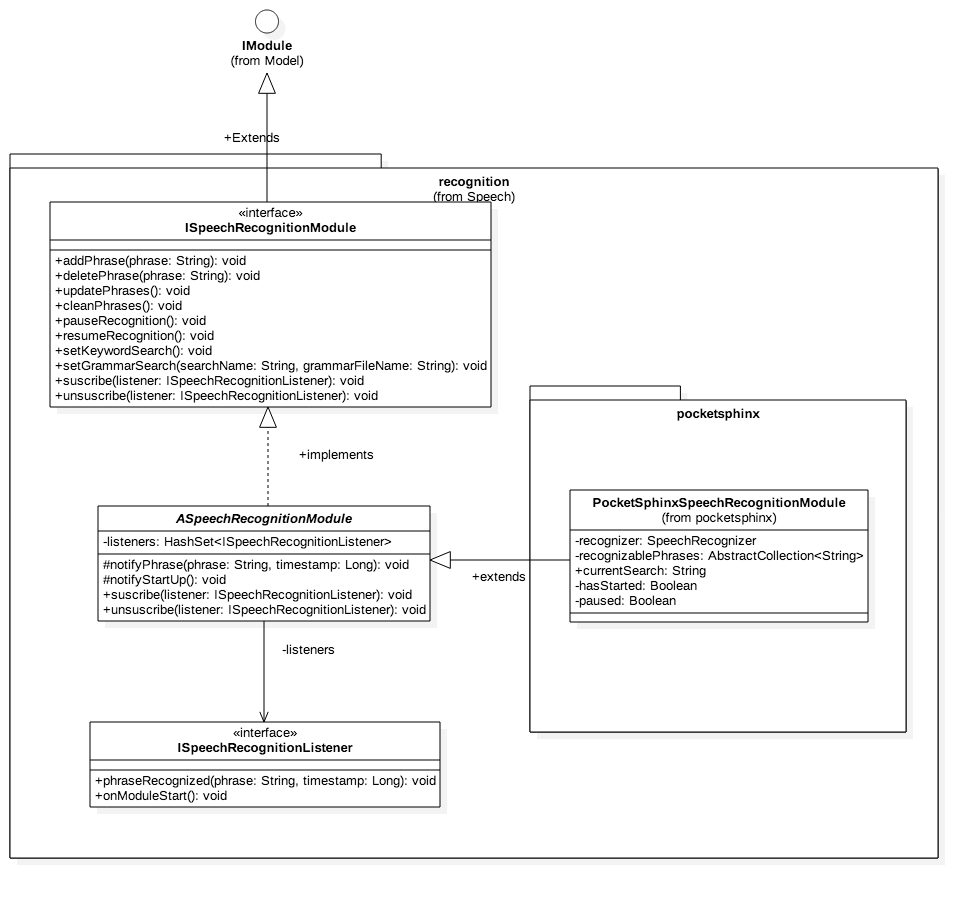
\includegraphics[width=1\linewidth]{imagenes/diagramas/SpeechRecognitionModule.png}
	\caption{Módulo SpeechRecognition}
	\label{fig:speech-recognition-module}
\end{figure}
El módulo recognition permite al usuario reconocer texto hablado de forma fácil.
Provee las Interfaces \textit{ISpeechRecognitionModule} y \textit{ISpeechRecognitionListener}, así cómo la clase abstracta \textit{ASpeechRecognitionModule}.

\textit{ISpeechRecognitionModule} ofrece la declaración de métodos de configuración del reconocedor de  voz y de suscripción de listeners.


Especificamente permite:
\begin{itemize}
 	\item Añadir y eliminar palabras reconocibles.
 	\item Actualizar el listado interno de frases
	\item Limpiar el listado interno
	\item Pausar y reanudar el reconocimiento
	\item Añadir búsquedas por gramática
	\item Utilizar búsqueda por palabras
 	 
\end{itemize}
\newpage


\textit{ISpeechRecognitionListener} es la interfaz que deben implementar las clases para ser notificados de los eventos que produce el módulo de reconocimiento.

Especificamente notifica cuando:
\begin{itemize}
	\item El reconocedor ha sido inicializado
	\item Una frase ha sido detectada
\end{itemize}

   


\textit{ASpeechRecognitionModule} es la clase abstracta que gestiona las tareas comunes a todas las implementaciones del modulo, a saber:

\begin{itemize}
	\item Mantener un listado de los listeners
	\item Suscribir y desuscribir listeners
	\item Notificar a los listeners de los diferentes eventos
\end{itemize}





\paragraph*{Pocketsphinx\\}


Se ha decidido realizar la implementación del módulo utilizando la librería CMU Sphinx \cite{cmusphinx}, desarrollada por la Universidad de Carnegie Mellon.
Específicamente se utiliza PocketSphinx, una versión de CMU Sphinx ligera, diseñada para su uso en sistemas embebidos.

PocketSphinx permite varios tipos de búsqueda diferentes, pero al contrario que las versiones más completas de la librería, sólo permite tener una búsqueda activa al mismo tiempo.
Entre los modos de búsqueda que ofrece se encuentran la búsqueda por Keywords y la búsqueda por Gramáticas, que son las que son ofrecidas por la interfaz del módulo. Adicionalmente PS también permite el uso de búsquedas por fonemas, pero no se ha contemplado su uso.

El módulo se llama  \textit{PocketSphinxSpeechRecognitionModule}, extiende \textit{ASpeechRecognitionModule} e implementa la interfaz \textit{RecognitionListener} que provee PocketSphinx.

La búsqueda por keywords permite al usuario definir, en tiempo de ejecución, una serie de palabras que podrán ser reconocidas, estas palabras deben estar contenidas en el diccionario del modelo fonético.

La búsqueda por gramática permite definir archivos de gramáticas en el formato  JSFG 1.0\cite{JSFGGrammar}, lo cual permite detectar construcciones más complejas de palabras.
%%todo Esto debería ir en el manual de usuario?
Para funcionar correctamente deben colocarse en el directorio assets/sync/ de la aplicación tanto el modelo fonético del idioma, como los archivos de gramáticas que se vayan a utilizar, todo archivo dentro de este directorio debe contar con un fichero de mismo nombre y extensión .md5 conteniendo un hash del original en su interior. Los archivos deben ser declarados dentro del fichero assets.lst.

Dado que el inicio del reconocedor de voz se realiza de manera asíncrona, es necesario notificar a la aplicación principal de cuando el módulo esta preparado, de lo contrario, llamar a una operación del mismo podría ser inseguro. Le arranque del módulo se notifica a través del método onModuleStart() que debe ser implementado por cualquier clase que vaya a utilizar el  módulo.


\subsubsection{Módulo Production}
\begin{figure}
	\centering
	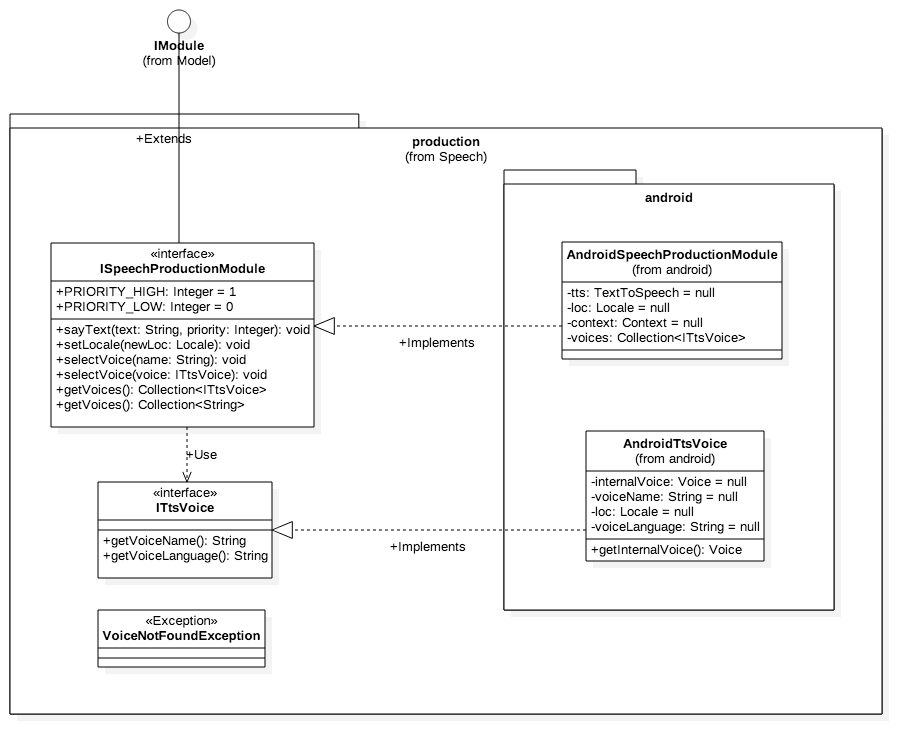
\includegraphics[width=1\linewidth]{imagenes/diagramas/SpeechProductionModule.png}
	\caption{Módulo SpeechProduction}
	\label{fig:speech-production-module}
\end{figure}

El módulo production permite al usuario producir voz a partir de texto de manera simple.
Provee la interfaces \textit{ISpeechProductionModule} y \textit{ITtsVoice}, así como la excepción \textit{VoiceNotFoundException}.
La primera contiene las declaraciones de los métodos del módulo en sí, la segunda provee una forma de representar las diferentes voces a utilizar por el módulo.

Las funcionalidades que provee la interfaz son:

\begin{itemize}
	\item Pronunciar un texto
	\item Cambiar la localización 
	\item Seleccionar voces
	\item Recuperar las voces disponibles
\end{itemize}

 


Implementación específica:

La implementación de la interfaz se ha realizado con las librerías del propio sistema Android (\textbf{android.speech.tts.TextToSpeech})

\newpage
\subsection{Paquete Touch}


\begin{figure}
	\centering
	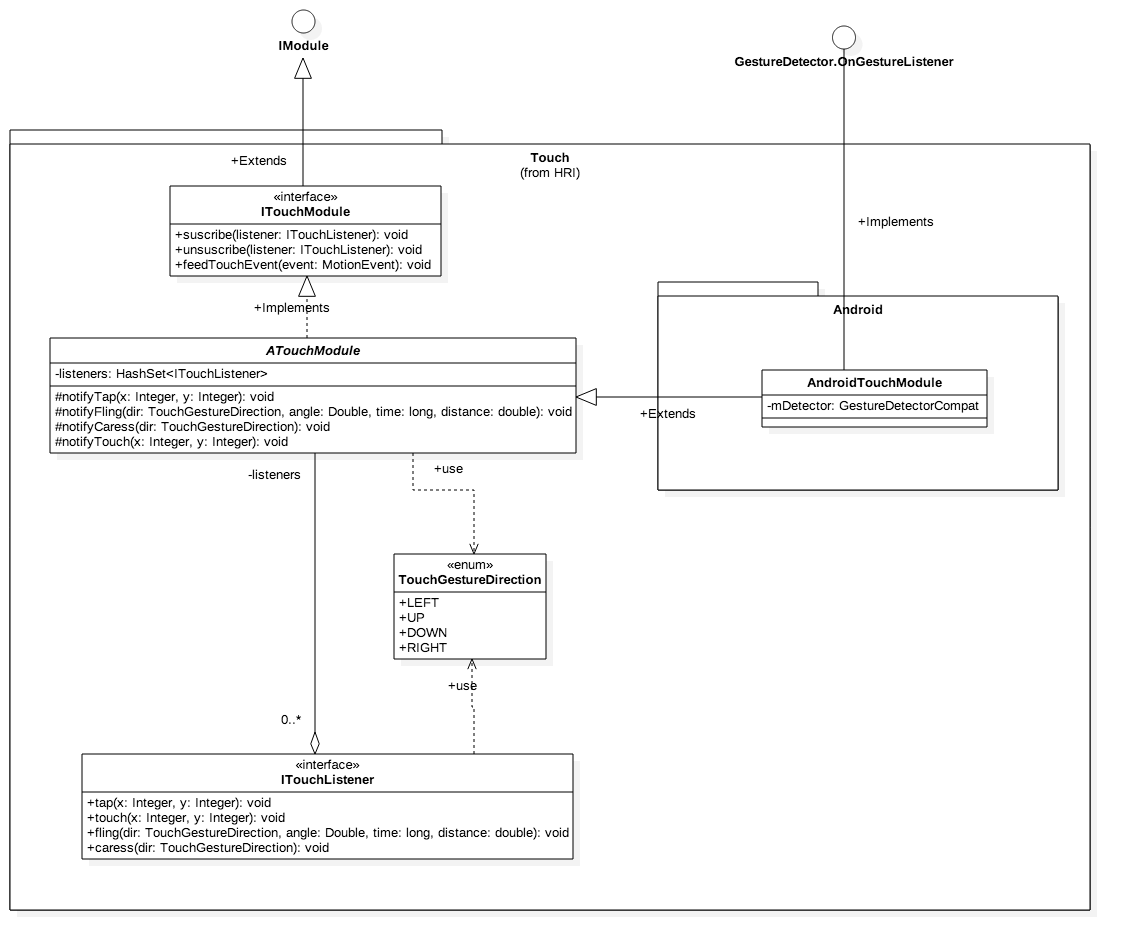
\includegraphics[width=1\linewidth]{imagenes/diagramas/TouchModule.png}
	\caption{Módulo Touch}
	\label{fig:touch-module}
\end{figure}


El subsistema Touch permite interacción con el robot en forma de gestos táctiles sobre la pantalla del teléfono. En su interior encontramos un único modulo, el módulo touch.

\subsubsection{Módulo Touch}
El módulo contiene las interfaces \textit{ITouchModule} e \textit{ITouchListener}, la clase abstracta \textit{ATouchModule} y por la clase enumerado \textit{TouchGestureDirection}.

\textit{ITouchListener} es la interfaz que debe implementar cualquier clase que quiera ser informada de los gestos táctiles que ocurran en la pantalla del dispositivo. Las acciones que se detectan son:

\begin{itemize}
	\item  Tap: Toque simple y rápido en la pantalla
	\item  Touch: Toque mantenido en la pantalla
	\item  Caress: Deslizamiento sobre la pantalla
	\item  Fling: Al terminar un deslizamiento de manera rápida
\end{itemize}


\textit{ITouchModule} es la interfaz que debe cualquier implementación del módulo. El único método remarcable de la misma es \textit{FeedTouchEvent}, en el cual se le pasan los eventos táctiles al módulo desde la aplicación principal, que debe sobrecargar el método \textit{OnTouchEvent} de la clase \textit{Activity}, esto es debido a que el módulo no puede extender la clase \textit{Activity}.

\paragraph*{Detección táctil de Android\\}


Para la implementación del módulo se escogió usar la clase \textit{GestureDetector} propia de Android, que provee de varios listeners para diferentes eventos táctiles.
Se han simplificado dichos eventos, para producir los definidos en \textit{ITouchListener}


\newpage

%%%%%%%%%%%%%%%%%%%%%%%%%%%%%%%%%%%%%%%%%%%%%%%%%%%%%%%%%%%%%%%%%%%%%%%%%%%%%%%%
\subsection{Paquete Sound}
Este subsistema contiene los módulos que realizan diversas tareas de reconocimiento de audio.  Han sido implementadas detección de tonos, notas musicales y palmadas.
\subsubsection{Módulo Sound Dispatcher}
\begin{figure}
	\centering
	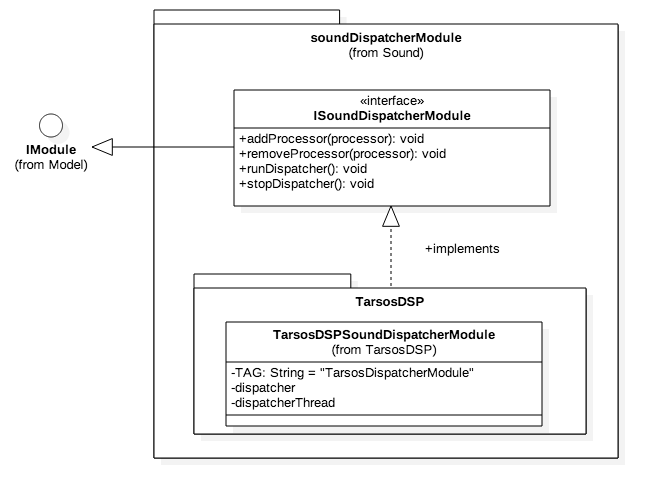
\includegraphics[width=1\linewidth]{imagenes/diagramas/SoundDispatcherModule.png}
	\caption{Módulo SoundDispatcher}
	\label{fig:sound-dispatcher-module}
\end{figure}
SoundDispatcher es un módulo de utilidad, necesario para el uso de los módulos implementados a partir de la librería TarsosDSP \cite{six2014tarsosdsp}.
Este módulo es el que se encarga de capturar el sonido del micrófono y segmentarlo en partes para su posterior procesado. Los distintos módulos se registran con sus procesadores en este módulo.
El paquete contiene en su interior \textit{ISoundDispatcherModule}, la interfaz del módulo, que permite
\begin{itemize}
	\item Añadir procesadores de audio
	\item Eliminar procesadores de audio
	\item Iniciar el procesado de audio
	\item Parar el procesado de audio
\end{itemize}
\textit{ASoundDispatcherModule} implementa \textit{ISoundDispatcherModule}, pese a estar vacía se conserva para mantener la estructura común de los módulos.
\paragraph*{TarsosDSP\\}
La implementación se realiza en el módulo \textit{TarsosDSPSoundDispatcherModule}, que extiende la clase \textit{ASoundDispatcherModule}.
En su interior se crea un objeto \textit{AudioDispatcher}, que se encarga del procesado del audio, y al que pueden añadirse distintos procesadores de audio.


\subsubsection{Módulo Pitch Detection}
\begin{figure}
	\centering
	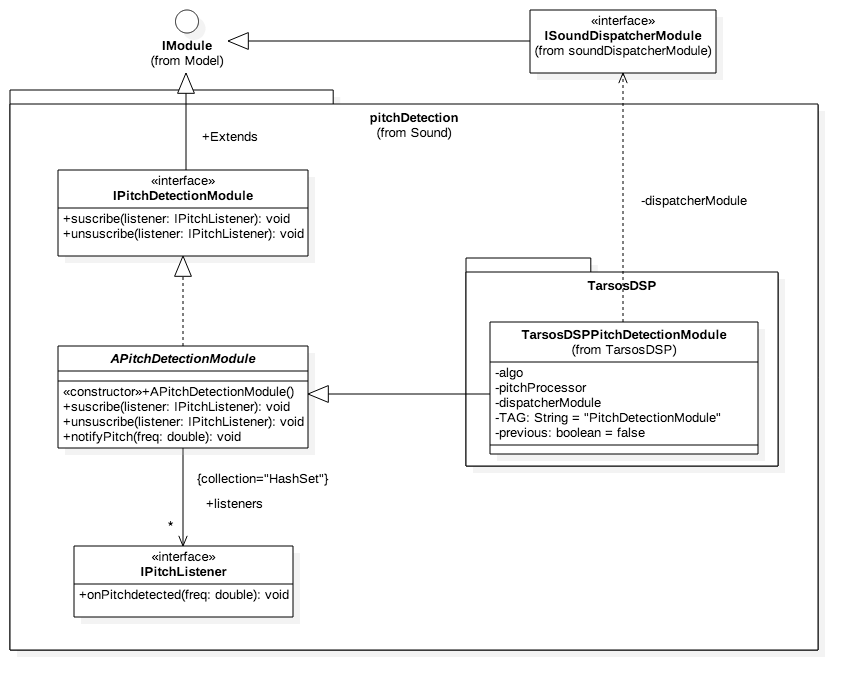
\includegraphics[width=1\linewidth]{imagenes/diagramas/PitchDetectionModule.png}
	\caption{Módulo PitchDetection}
	\label{fig:pitch-detection-module}
\end{figure}
PitchDetection permite detectar la frecuencia en Hertzios de sonidos, es utilizado, por ejemplo en el módulo de detección de notas musicales.
En su interior encontramos la interfaz \textit{IPitchDetectionModule} y la clase abstracta \textit{APitchDetectionModule}, que gestionan la suscripción de listeners a los eventos. También se encuentra \textit{IPitchListener}, que debe ser implementada por cualquier clase que desee recibir notificaciones del módulo de detección de tonos.

\paragraph*{TarsosDSP \\}
La implementación del módulo se ha realizado en la clase \textit{TarsosDSPPitchDetectionModule}. Esta implementación depende del módulo SoundDispatcher, ya que en su inicialización se registra a si mismo en el susodicho modulo.
%TODO No se muy bien como redactar esto
Esta implementación utiliza el algoritmo YIN \cite{de_YINa_f2002} para la detección de frecuencias. La implementación del algoritmo viene dada por la propia librería TarsosDSP. El módulo genera un evento con la frecuencia cuando un sonido es detectado, y al terminar la detección devuelve un -1.

\subsubsection{Módulo Note Detection}
\begin{figure}
	\centering
	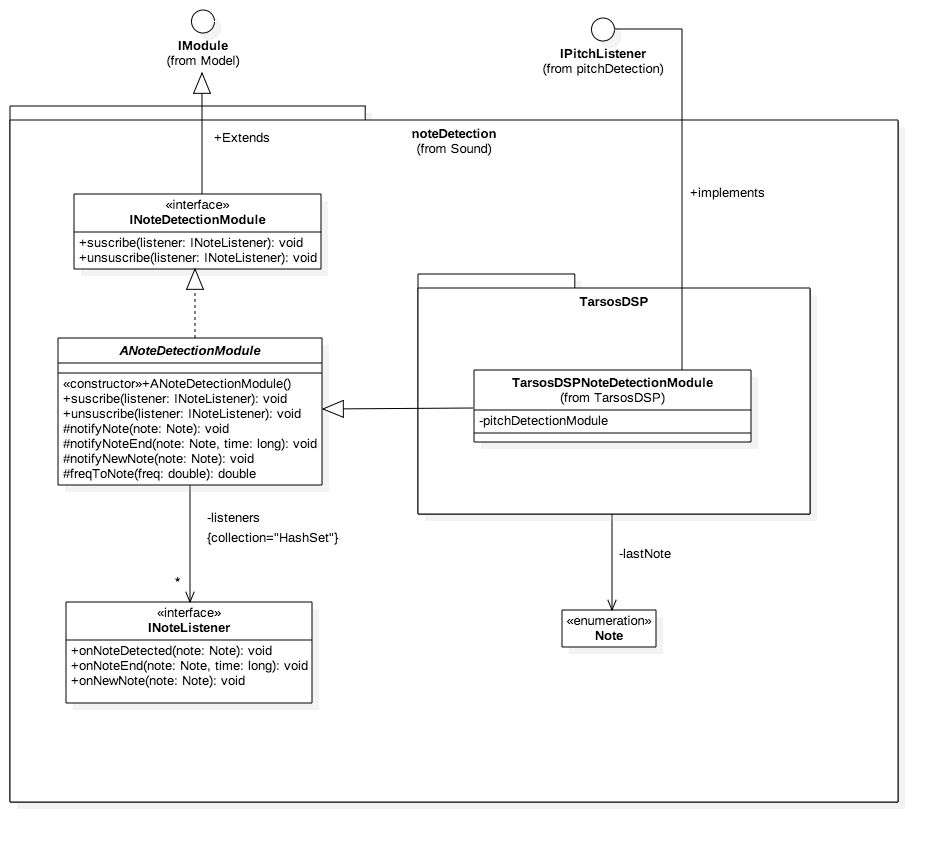
\includegraphics[width=1\linewidth]{imagenes/diagramas/NoteDetectionModule.png}
	\caption{Módulo NoteDetection}
	\label{fig:note-detection-module}
\end{figure}
El módulo NoteDetection busca proporcionar una manera simple de detectar notas musicales. Depende directamente del módulo PitchDetection, del cual obtiene la frecuencia que traduce en notas musicales.
En su interior encontramos la interfaz del módulo \textit{INoteDetectionModule}, la clase abstracta \textit{ANoteDetectionModule}, que además de la gestión de listeners provee un método de conversión de frecuencias a notas, la interfaz \textit{INoteListener} que recibe notificaciones al:
\begin{itemize}
	\item Comenzar una nota
	\item Detectar una nota
	\item Terminar una nota
\end{itemize}
 Toda clase que desee recibir los eventos producidos por el módulo debe implementar esta interfaz.
 Por último en el paquete encontramos una clase \textit{Note} que se utiliza como representación de las notas musicales. Este enumerado contiene la información del índice de la conversión de notas, la nota musical en formato anglosajón, y la octava a la que pertenece la nota.
 
 \paragraph*{TarsosDSP\\}%todo realmente no usa la libreria directamente
 
 \textit{TarsosDSPNoteDetectionModule} extiende \textit{ANoteDetectionModule} e implementa \textit{IPitchListener}. Simplemente convierte los tonos detectados a notas musicales, filtra las notas desafinadas y controla los inicios y finalizaciones de las notas, generando eventos de los cuales serán notificados los listeners.
\subsubsection{Módulo Clap Detection}
\begin{figure}
	\centering
	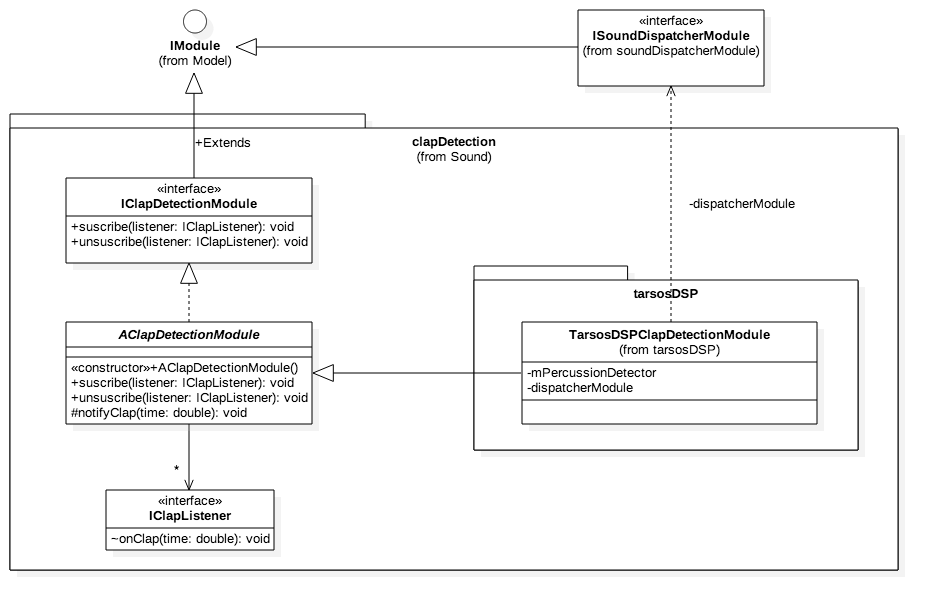
\includegraphics[width=1\linewidth]{imagenes/diagramas/ClapDetectionModule.png}
	\caption{Módulo ClapDetection}
	\label{fig:clap-detection-module}
\end{figure}
El módulo ClapDetection permite detectar ruidos percusivos tales como palmadas. Igual que el PitchDetection, depende directamente del módulo SoundDispatcher para su funcionamiento. En su interior se encuentra la interfaz del módulo, \textit{IClapDetectionModule}, la clase abstracta \textit{AClapDetectionModule} y la interfaz del listener, \textit{IClapListener}. Las clases que implementen este listener recibirán una notificación cada vez que se detecte una palmada.
\paragraph*{TarsosDSP\\} 
La implementación del módulo, contenida en \textit{TarsosDSPClapDetectionModule}, emplea el objeto provisto por la librería TarsosDSP \textit{PercussionOnsetDetector}, que es registrado en el \textit{DispatcherModule} activo en ese momento. Este objeto permite la detección de sonidos percusivos, como palmadas de una forma sencilla.

\subsubsection{Módulo NoteGenerator}
\begin{figure}
	\centering
	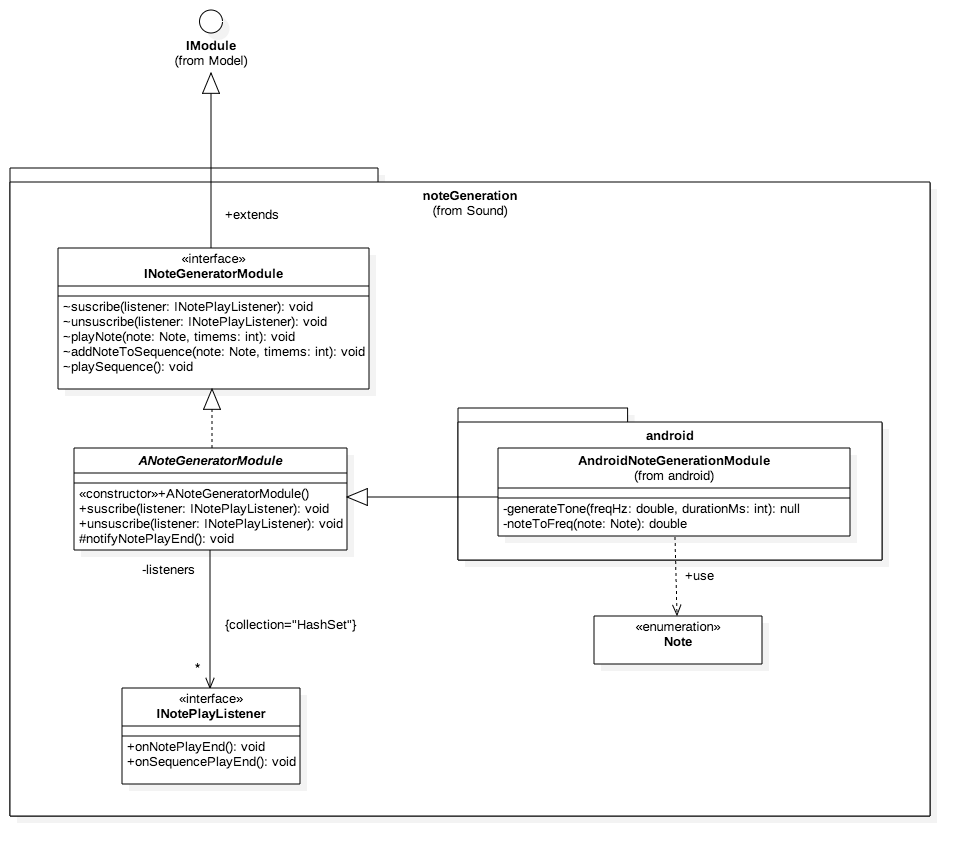
\includegraphics[width=1\linewidth]{imagenes/diagramas/NoteGenerationModule.png}
	\caption{Módulo NoteGenerator}
	\label{fig:note-generator-module}
\end{figure}
El módulo NoteGenerator provee una forma de sintetizar tonos musicales y hacer sonar secuencias de notas.
En su interior se encuentra la interfaz del módulo \textit{INoteGeneratorModule} que define las funcionalidades del módulo, la clase abstracta \textit{ANoteGeneratorModule} que gestiona la suscripción a los listeners. La interfaz del listener se encuentra en \textit{INotePlayListener} y su finalidad es notificar cuando una nota o una secuencia de notas termina de reproducirse. La clase \textit{Note} es la representación de las notas musicales en el sistema, contiene la nota, el índice y la octava.

\paragraph*{Android\\}

La implementación especifica del módulo se encuentra en AndroidNoteGeneratorModule y se ha realizado mediante la clase \textit{AudioTrack}. El objeto \textit{AudioTrack} se crea sample a sample utilizando la ecuación de una onda senoidal de la frecuencia de la nota requerida. La reproducción de secuencias se implementa mediante el uso de las clases \textit{Timer} y \textit{TimerTask}


\subsubsection{Módulo EmotionSound}
\begin{figure}
	\centering
	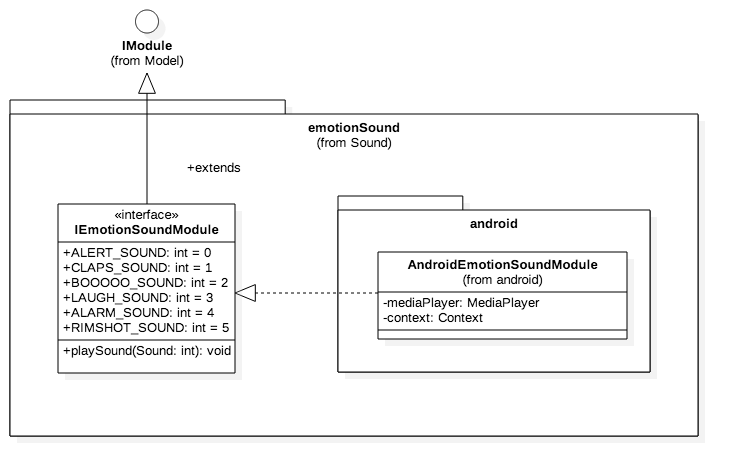
\includegraphics[width=1\linewidth]{imagenes/diagramas/EmotionSoundModule.png}
	\caption{Módulo EmotionSound}
	\label{fig:emotion-sound-module}
\end{figure}
El módulo EmotionSound busca proporcionar una manera de reproducir una serie de sonidos prefijados para expresar diferentes emociones.
La interfaz del módulo esta definida en \textit{IEmotionSoundModule}, y en ella están definidos, en forma de constantes, los sonidos utilizables.
Los sonidos se encuentran en el directorio raw de la carpeta res del paquete Sound.
\paragraph*{Android\\}

La implementación de este módulo se ha realizado mediante la clase \textit{MediaPlayer} provista por la API de Android, que permite reproducir diferentes recursos audiovisuales. El módulo está definido en la clase \textit{AndroidEmotionSoundModule}.



\newpage
%%%%%%%%%%%%%%%%%%%%%%%%%%%%%%%%%%%%%%%%%%%%%%%%%%%%%%%%%%%%%%%%%%%%%%%%%%%%%%%%
\subsection{Paquete Vision}
Este subsistema contiene los diferentes módulos de captura y procesado de imagen
\subsubsection{Módulo Basic Camera}
\begin{figure}
	\centering
	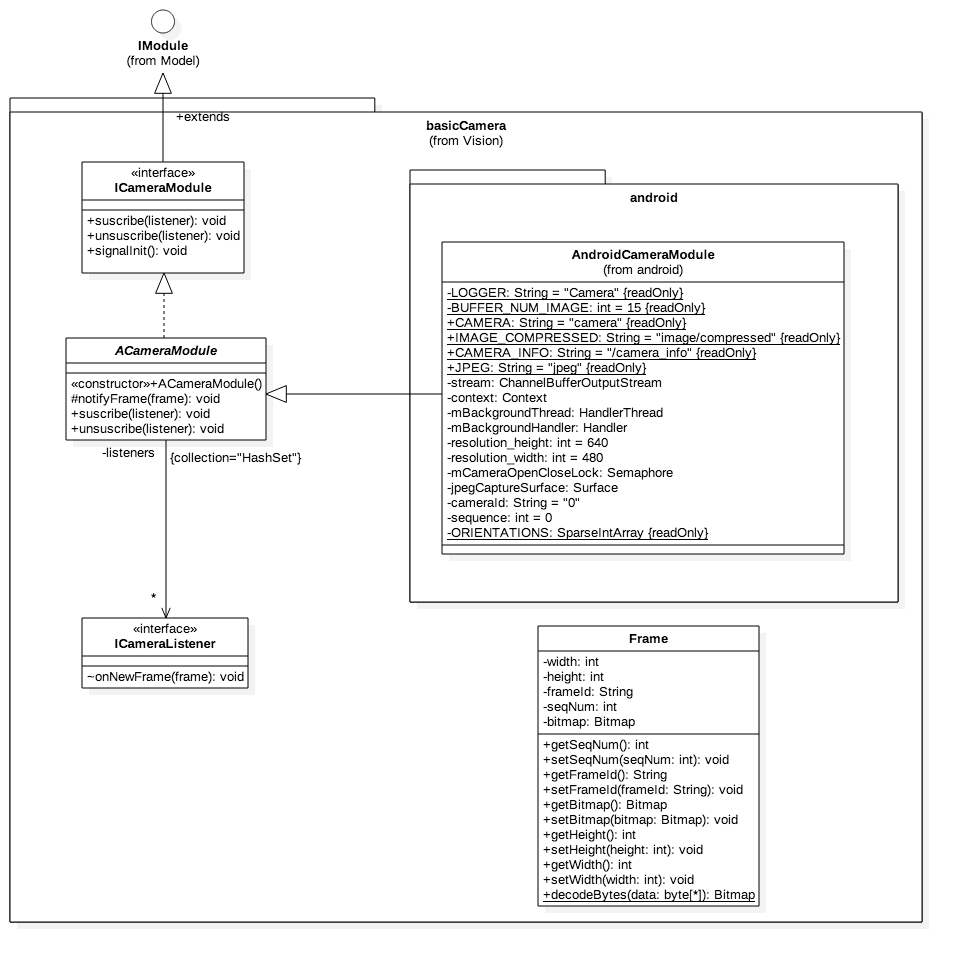
\includegraphics[width=1\linewidth]{imagenes/diagramas/BasicCameraModule.png}
	\caption{Módulo BasicCamera}
	\label{fig:basic-camera-module}
\end{figure}
Este es el módulo básico de cámara, del cual hacen uso el resto de módulos de procesado de imagen. Este modulo produce un stream constante de imágenes, que no deben ser necesariamente mostradas, capturadas de la cámara frontal del dispositivo y notifica a los listeners suscritos.
La interfaz del módulo se encuentra en \textit{ICameraModule}, la clase abstracta que gestiona los listeners en \textit{ACameraModule} y la interfaz del listener en el que se notifica la captura de las imágenes en \textit{ICameraListener}. Además, el modulo proporciona una clase Frame, que representa a las imágenes capturadas con sus características.

\paragraph*{Android Camera2\\}
Para realizar la implementación del módulo se ha empleado la clase \textit{Camera2} que proporciona Android. Esta implementación permite obtener el stream mencionado anteriormente sin mostrar las imágenes en la pantalla, pero produce una velocidad de captura de imágenes baja, de alrededor de dos cuadros por segundo en el smartphone de pruebas (BQ Aquaris M5) variando de teléfono a teléfono.
\subsubsection{Módulo Face Detection}
\begin{figure}
	\centering
	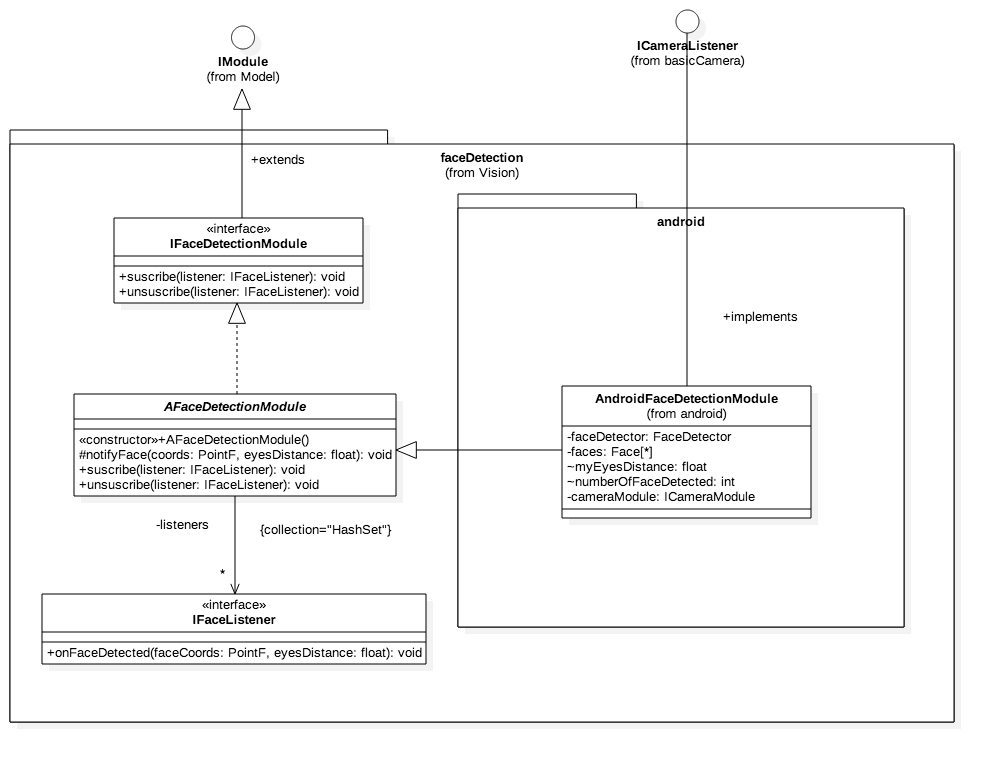
\includegraphics[width=1\linewidth]{imagenes/diagramas/FaceDetectionModule.png}
	\caption{Módulo FaceDetection}
	\label{fig:face-detection-module}
\end{figure}
El módulo FaceDetection permite detectar caras en los frames producidos por el módulo BasicCamera. La interfaz del módulo es \textit{IFaceDetectionModule} y su clase abstracta \textit{AFaceDetectionModule}. El listener que debe ser implementado por la clase que utilice el módulo es \textit{IFaceListener}, que notifica de las coordenadas del centro de la cara y de la distancia entre ojos cuando una cara es detectada. Solo se contempla la detección de una cara al mismo tiempo.

\paragraph*{Android FaceDetector\\}
Para implementar este módulo se ha empleado la clase \textit{FaceDetector} provista por el paquete Media de Android, el módulo se llama \textit{AndroidFaceDetectionModule}.
\newpage

\subsubsection{Módulo ColorDetector}
\begin{figure}
	\centering
	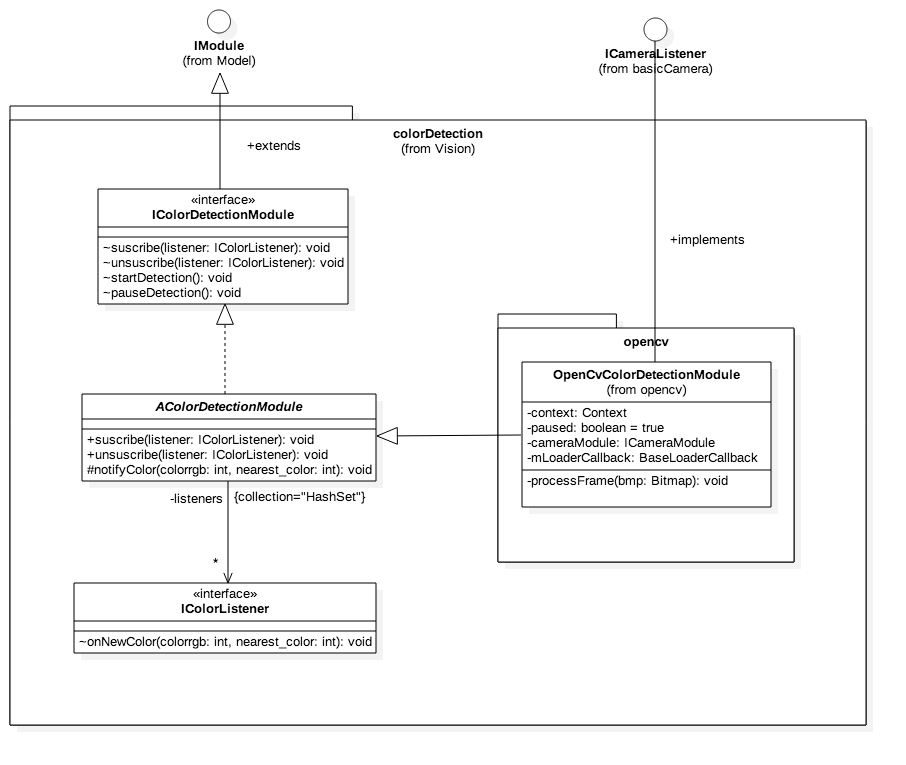
\includegraphics[width=1\linewidth]{imagenes/diagramas/ColorDetectionModule.png}
	\caption{Módulo ColorDetection}
	\label{fig:color-detection-module}
\end{figure}
Este módulo provee la funcionalidad de detección de colores sobre fondos con alto contraste. La interfaz del módulo se puede encontrar en \textit{IColorDetectionModule}, la clase abstracta \textit{AColorDetectionModule} gestiona los listeners en los que será notificada la detección de los colores. La interfaz de dicho listener se encuentra en la clase \textit{IColorListener} y debe ser implementada por toda clase que desee recibir las notificaciones de los colores.

\paragraph{OpenCV}

Para realizar la implementación de este módulo se ha empleado la librería OpenCV\cite{opencv} una de las más usadas en visión por computador. Este módulo, contenido en \textit{OpenCVColorDetectionModule} realiza los siguientes pasos para la detección de colores:
\begin{itemize}
	\item Detección de bordes mediante el algoritmo de Canny, obteniendo el contorno con mayor area.
	\item Creación de una máscara binaria con el area detectada
	\item Conversión de la imagen original al espacio de color HSV
	\item Media de color en los pixeles no nulos en el canal H de la imagen resultante de un AND entre la máscara y ma imagen convertida
	\item Clasificación del color detectado
\end{itemize}

%%%%%%%%%%%%%%%%%%%%%%%%%%%%%%%%%%%%%%%%%%%%%%%%%%%%%%%%%%%%%%%%%%%%%%%%%%%%%%%%
\subsection{Paquete Messaging}
El subsistema Messaging aglomera las diferentes opciones de comunicación por mensajería de texto.
\subsubsection{Módulo email}
\begin{figure}
	\centering
	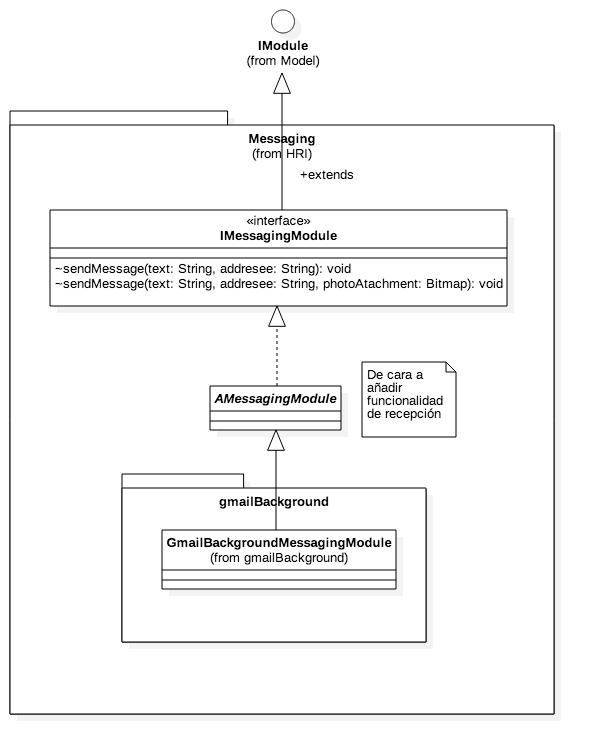
\includegraphics[width=0.7\linewidth]{imagenes/diagramas/MessagingModule.png}
	\caption{Módulo Email}
	\label{fig:email-module}
\end{figure}
El módulo Email permite al usuario la comunicación mediante correo electrónico, pudiendo mandar tanto texto como imágenes, por ejemplo, las capturadas con el módulo \textit{BasicCamera}.

\paragraph*{GmailBackground\\}
Para implementar el módulo, se ha empleado la librería GmailBackGround \cite{gmailbg}, que permite el envío de mensajes de correo electrónico con una cuenta de Gmail. El módulo se encuentra en la clase \textit{GmailBackgroundMessagingModule}.
\newpage









 \chapter{Resultados}
\label{chap:results}
\vspace{0.5cm}

%%%%%%%%%%%%%%%%%%%%%%%%%%%%%%%%%%%%%%%%%%%%%%%%%%%%%%%%%%%%%%%%%%%%%%%%%%%%%%%%
% Objetivo: Exponer los resultados objetivos del sistema                       %
%%%%%%%%%%%%%%%%%%%%%%%%%%%%%%%%%%%%%%%%%%%%%%%%%%%%%%%%%%%%%%%%%%%%%%%%%%%%%%%%

 
\lettrine{E}{n} este capítulo se expondrán los resultados y el funcionamiento de los módulos desarrollados en este trabajo mediante tres aplicaciones de ejemplo.
\section{Ejemplos de uso}
\subsection{Simon dice músical}
\subsection{Robobo Vigilante}
\subsection{Robobo Mascota}


\section{Problemas conocidos}
\begin{itemize}
	\item La tasa de refresco del módulo \textit{BasicCamera} es baja y varía mucho entre terminales móviles.
	\item El \textit{ColorDetectionModule} puede confundirse si el fondo no es homogéneo, se recomienda usar tarjetas con colores sobre fondo blanco.
	\item El \textit{EmailModule} puede causar el bloqueo de la cuenta de Gmail si esta no es configurada previamente para usar mediante IMAP.
	\item El \textit{TouchModule} requiere el paso explícito de los TouchEvents de la actividad en pantalla.
\end{itemize}
\label{sec:known_issues}
    


 \chapter{Conclusiones}
\label{chap:conclusiones}
\vspace{0.5cm}

%%%%%%%%%%%%%%%%%%%%%%%%%%%%%%%%%%%%%%%%%%%%%%%%%%%%%%%%%%%%%%%%%%%%%%%%%%%%%%%%
% Objetivo: Contar cómo está ahora el proyecto, si ha merecido la              %
%           pena, lo que se ha aprendido, si se aplicaría de nuevo, etc.       %
%%%%%%%%%%%%%%%%%%%%%%%%%%%%%%%%%%%%%%%%%%%%%%%%%%%%%%%%%%%%%%%%%%%%%%%%%%%%%%%%


\section{Trabajo Futuro}


 %%%%%%%%%%%%%%%%%%%%%%%%%%%%%%%%%%%%%%%%
 % Apéndices, glosarios y bibliografía  %
 %%%%%%%%%%%%%%%%%%%%%%%%%%%%%%%%%%%%%%%%
 \appendix
 \newpage
%%\chapter{Diagramas}
%%\label{chap:diagrams}
 
\chapter{Instalación}
\label{chap:installation}
\chapter{Manual de uso}
\label{chap:usage}

\newpage
\thispagestyle{empty}


 \nocite*
 \bibliography{bibliography}
 \bibliographystyle{IEEEtran}


\end{document}

%%%%%%%%%%%%%%%%%%%%%%%%%%%%%%%%%%%%%%%%%%%%%%%%%%%%%%%%%%%%%%%%%%%%%%%%%%%%%%%%
